%% (Master) Thesis template
% Template version used: v2
%
% Largely adapted from Adrian Nievergelt's template for the ADPS
% (lecture notes) project.

%% We use the memoir class because it offers many easy to use features.
% Template v2 fixes:
% Removed titlepage from options: LaTeX Warning: Unused global option(s): [titlepage].
% Electronic version that does not waste space
% \documentclass[11pt,a4paper,openany,oneside]{memoir}
% Printable version that does waste space (but people like it), uncomment for printing
\documentclass[11pt,a4paper]{memoir}

%% Packages
%% ========

%% LaTeX Font encoding -- DO NOT CHANGE
\usepackage[OT1]{fontenc}
\usepackage{subcaption}
\usepackage{float}
\usepackage{algorithm}
\usepackage{algpseudocode}
%% Babel provides support for languages.  'english' uses British
%% English hyphenation and text snippets like "Figure" and
%% "Theorem". Use the option 'ngerman' if your document is in German.
%% Use 'american' for American English.  Note that if you change this,
%% the next LaTeX run may show spurious errors.  Simply run it again.
%% If they persist, remove the .aux file and try again.
\usepackage[english]{babel}

%% Input encoding 'utf8'. In some cases you might need 'utf8x' for
%% extra symbols. Not all editors, especially on Windows, are UTF-8
%% capable, so you may want to use 'latin1' instead.
\usepackage[utf8]{inputenc}

%% This changes default fonts for both text and math mode to use Herman Zapfs
%% excellent Palatino font.  Do not change this.
\usepackage[sc]{mathpazo}

%% The AMS-LaTeX extensions for mathematical typesetting.  Do not
%% remove.
\usepackage{amsmath,amssymb,amsfonts,mathrsfs}

%% NTheorem is a reimplementation of the AMS Theorem package. This
%% will allow us to typeset theorems like examples, proofs and
%% similar.  Do not remove.
%% NOTE: Must be loaded AFTER amsmath, or the \qed placement will
%% break
\usepackage[amsmath,thmmarks]{ntheorem}

%% LaTeX' own graphics handling
\usepackage{graphicx}

%% We unfortunately need this for the Rules chapter.  Remove it
%% afterwards; or at least NEVER use its underlining features.
\usepackage{soul}

%% This allows you to add .pdf files. It is used to add the
%% declaration of originality.
\usepackage{pdfpages}

\usepackage{minted}

%% Some more packages that you may want to use.  Have a look at the
%% file, and consult the package docs for each.
%% See the TeXed file for more explanations

%% [OPT] Multi-rowed cells in tabulars
%\usepackage{multirow}

%% Make document internal hyperlinks wherever possible. (TOC, references)
%% This MUST be loaded before cleveref
\usepackage[linkcolor=black,colorlinks=true,citecolor=black,filecolor=black]{hyperref}

%% [REC] Intelligent cross reference package. This allows for nice
%% combined references that include the reference and a hint to where
%% to look for it.
%% Template v2: cleveref already recognizes what is being referenced - one does not need to write Fig./Sec.
% \usepackage{varioref}. Capitalization is prefered in CS
\usepackage[capitalise]{cleveref}

%% [OPT] Easily changeable quotes with \enquote{Text}
\usepackage[german=swiss]{csquotes}

%% Template v2: this prevents warning "Package fmtcount Warning: \ordinal already defined use \FCordinal instead. on input line". See https://tex.stackexchange.com/questions/162353/memoir-class-conflict-with-datetime#comment371926_162358
\let\ordinal\relax
%% [REC] Format dates and time depending on locale
\usepackage{datetime}

%% [OPT] Provides a \cancel{} command to stroke through mathematics.
%\usepackage{cancel}

%% [NEED] This allows for additional typesetting tools in mathmode.
%% See its excellent documentation.
\usepackage{mathtools}

%% [ADV] Conditional commands
%\usepackage{ifthen}

%% [OPT] Manual large braces or other delimiters.
%\usepackage{bigdelim, bigstrut}

%% [REC] Alternate vector arrows. Use the command \vv{} to get scaled
%% vector arrows.
\usepackage[h]{esvect}

%% [NEED] Some extensions to tabulars and array environments.
\usepackage{array}

%% [OPT] Postscript support via pstricks graphics package. Very
%% diverse applications.
%\usepackage{pstricks,pst-all}

%% [?] This seems to allow us to define some additional counters.
%\usepackage{etex}

%% [ADV] XY-Pic to typeset some matrix-style graphics
%\usepackage[all]{xy}

%% [OPT] This is needed to generate an index at the end of the
%% document.
%\usepackage{makeidx}

%% [OPT] Fancy package for source code listings.  The template text
%% needs it for some LaTeX snippets; remove/adapt the \lstset when you
%% remove the template content.
\usepackage{listings}
\lstset{language=TeX,basicstyle={\normalfont\ttfamily}}

% Template v2 fixes: this is an old package, microtype is superior + fixes an error
%% [REC] Fancy character protrusion.  Must be loaded after all fonts.
\usepackage[activate]{microtype}
% \usepackage[activate]{pdfcprot}  % causes the compilation error

%% [REC] Nicer tables.  Read the excellent documentation.
\usepackage{booktabs}


%% Our layout configuration.  DO NOT CHANGE.
%% Memoir layout setup

%% NOTE: You are strongly advised not to change any of them unless you
%% know what you are doing.  These settings strongly interact in the
%% final look of the document.

% Dependencies
\usepackage{eth-template/ETHlogo}

% Turn extra space before chapter headings off.
\setlength{\beforechapskip}{0pt}

\nonzeroparskip
\parindent=0pt
\defaultlists

% Chapter style redefinition
\makeatletter

\if@twoside
  \pagestyle{Ruled}
  \copypagestyle{chapter}{Ruled}
\else
  \pagestyle{ruled}
  \copypagestyle{chapter}{ruled}
\fi
\makeoddhead{chapter}{}{}{}
\makeevenhead{chapter}{}{}{}
\makeheadrule{chapter}{\textwidth}{0pt}
\copypagestyle{abstract}{empty}
\copypagestyle{something}{empty}


\makechapterstyle{bianchimod}{%
  \chapterstyle{default}
  \renewcommand*{\chapnamefont}{\normalfont\Large\sffamily}
  \renewcommand*{\chapnumfont}{\normalfont\Large\sffamily}
  \renewcommand*{\printchaptername}{%
    \chapnamefont\centering\@chapapp}
  \renewcommand*{\printchapternum}{\chapnumfont {\thechapter}}
  \renewcommand*{\chaptitlefont}{\normalfont\huge\sffamily}
  \renewcommand*{\printchaptertitle}[1]{%
    \hrule\vskip\onelineskip \centering \chaptitlefont\textbf{\vphantom{gyM}##1}\par}
  \renewcommand*{\afterchaptertitle}{\vskip\onelineskip \hrule\vskip
    \afterchapskip}
  \renewcommand*{\printchapternonum}{%
    \vphantom{\chapnumfont {9}}\afterchapternum}}

% Use the newly defined style
\chapterstyle{bianchimod}

\setsecheadstyle{\Large\bfseries\sffamily}
\setsubsecheadstyle{\large\bfseries\sffamily}
\setsubsubsecheadstyle{\bfseries\sffamily}
\setparaheadstyle{\normalsize\bfseries\sffamily}
\setsubparaheadstyle{\normalsize\itshape\sffamily}
\setsubparaindent{0pt}

% Set captions to a more separated style for clearness
\captionnamefont{\sffamily\bfseries\footnotesize}
\captiontitlefont{\sffamily\footnotesize}
\setlength{\intextsep}{16pt}
\setlength{\belowcaptionskip}{1pt}

% Set section and TOC numbering depth to subsection
\setsecnumdepth{subsection}
\settocdepth{subsection}

%% Titlepage adjustments
\pretitle{\vspace{0pt plus 0.7fill}\begin{center}\HUGE\sffamily\bfseries}
\posttitle{\end{center}\par}
\preauthor{\par\begin{center}\let\and\\\Large\sffamily}
\postauthor{\end{center}}
\predate{\par\begin{center}\Large\sffamily}
\postdate{\end{center}}

\def\@advisors{}
\newcommand{\advisors}[1]{\def\@advisors{#1}}
\def\@department{}
\newcommand{\department}[1]{\def\@department{#1}}
\def\@thesistype{}
\newcommand{\thesistype}[1]{\def\@thesistype{#1}}

\renewcommand{\maketitlehooka}{\noindent\ETHlogo[2in]}

\renewcommand{\maketitlehookb}{\vspace{1in}%
  \par\begin{center}\Large\sffamily\@thesistype\end{center}}

\renewcommand{\maketitlehookd}{%
  \vfill\par
  \begin{flushright}
    \sffamily
    \@advisors\par
    \@department, ETH Z\"urich
  \end{flushright}
}

\checkandfixthelayout

\setlength{\droptitle}{-48pt}

\makeatother

% This defines how theorems should look. Best leave as is.
\theoremstyle{plain}
\setlength\theorempostskipamount{0pt}

%%% Local Variables:
%%% mode: latex
%%% TeX-master: "thesis"
%%% End:


%% Theorem environments.  You will have to adapt this for a German
%% thesis.
%% Theorem-like environments

%% This can be changed according to language. You can comment out the ones you
%% don't need.

\numberwithin{equation}{chapter}

%% German theorems
%\newtheorem{satz}{Satz}[chapter]
%\newtheorem{beispiel}[satz]{Beispiel}
%\newtheorem{bemerkung}[satz]{Bemerkung}
%\newtheorem{korrolar}[satz]{Korrolar}
%\newtheorem{definition}[satz]{Definition}
%\newtheorem{lemma}[satz]{Lemma}
%\newtheorem{proposition}[satz]{Proposition}

%% English variants
\newtheorem{theorem}{Theorem}[chapter]
\newtheorem{example}[theorem]{Example}
\newtheorem{remark}[theorem]{Remark}
\newtheorem{corollary}[theorem]{Corollary}
\newtheorem{definition}[theorem]{Definition}
\newtheorem{lemma}[theorem]{Lemma}
\newtheorem{proposition}[theorem]{Proposition}

%% Proof environment with a small square as a "qed" symbol
\theoremstyle{nonumberplain}
\theorembodyfont{\normalfont}
\theoremsymbol{\ensuremath{\square}}
\newtheorem{proof}{Proof}
%\newtheorem{beweis}{Beweis}


%% Helpful macros.
%% Custom commands
%% ===============

%% Special characters for number sets, e.g. real or complex numbers.
\newcommand{\C}{\mathbb{C}}
\newcommand{\K}{\mathbb{K}}
\newcommand{\N}{\mathbb{N}}
\newcommand{\Q}{\mathbb{Q}}
\newcommand{\R}{\mathbb{R}}
\newcommand{\Z}{\mathbb{Z}}
\newcommand{\X}{\mathbb{X}}

%% Fixed/scaling delimiter examples (see mathtools documentation)
\DeclarePairedDelimiter\abs{\lvert}{\rvert}
\DeclarePairedDelimiter\norm{\lVert}{\rVert}

%% Use the alternative epsilon per default and define the old one as \oldepsilon
\let\oldepsilon\epsilon
\renewcommand{\epsilon}{\ensuremath\varepsilon}

%% Also set the alternate phi as default.
\let\oldphi\phi
\renewcommand{\phi}{\ensuremath{\varphi}}


%% use code instead of texttt
\newcommand{\code}[1]{\texttt{#1}}

% Template v2: BibLaTeX with Biber backend are in my opinion best maintainable citation configurations. IEEE style is common in CS.
% Bibliography
\usepackage[
bibstyle=ieee,
citestyle=numeric,
isbn=true,
doi=true,
sorting=none,
url=true,
% defernumbers=true,
bibencoding=utf8,
backend=biber
]{biblatex} %Imports BibLaTeX package
\addbibresource{refs.bib} %Import the bibliography file

%% Document information
%% ====================

\title{Exploring the Correlation between Transactional Bugs and Isolation Levels}
\author{Theodor Moroianu}
\thesistype{Master Thesis}
\advisors{Advisors: Dr.\ Si Liu, Prof.\ Dr.\ David Basin}
\department{Department of Computer Science}
\date{December 3, 2024}


\definecolor{bg}{rgb}{0.95,0.95,0.95}

\begin{document}

\frontmatter

%% Title page is autogenerated from document information above.  DO
%% NOT CHANGE.
\begin{titlingpage}
  \calccentering{\unitlength}
  \begin{adjustwidth*}{\unitlength-24pt}{-\unitlength-24pt}
    \maketitle
  \end{adjustwidth*}
\end{titlingpage}

%% The abstract of your thesis.  Edit the file as needed.
\begin{abstract}

This thesis aims to uncover potential correlations between transactional

%   This thesis aims to understand different trade-offs between current distributed transaction protocols. Specifically, we focus on two widely used concurrency control levels: Causal Consistency and Snapshot Isolation. 

%   First, we aim to understand the different trade-offs between theoretical impossibility results under Causal Consistency: SNOW, NOCS, and NOC-NOC. NOC-NOC is a state-of-the-art concurrency control impossibility result. There are algorithms guided by NOC-NOC. The fundamental rationale behind these algorithms is to move the burdens from the network communication side to the local computation side. We thus conjecture that there are corner cases when local computation itself becomes the new system bottleneck, and thus algorithms guided by NOC-NOC will become sub-optimal. We experiment with a wide range of experiment settings, and the results show that the above conjecture does not hold. The possible explanation is that under current hardware settings, the network communication is much slower than the local computation, and moving the system burden to the local computation is generally a wise choice.


% Second, we focus on improving the efficiency of distributed concurrency control of Snapshot Isolation practically. The key idea behind our protocol is that as the current hardware improves, transactions will practically satisfy the snapshot isolation guarantee in most cases. Many existing protocols incur too much overhead checking whether transactions satisfy the snapshot isolation conditions. Our experiments show that our new distributed snapshot isolation protocols outperform the state-of-the-art.
  
\end{abstract}

\newpage

\section*{Acknowledgement}
TODO: Change.
I am incredibly grateful for having the opportunity to do my master's thesis in the Information Security Group. First and foremost, I would like to express my deepest thanks to Prof. Dr. David Basin. I am also profoundly grateful to my advisor, Dr. Si Liu, for the time we spent discussing the project's progress. I thank him for so many valuable suggestions and advice he gave to me. My master's thesis was partly built on Luca Multazzu's previous master's thesis. I thank him for his detailed help. Although he already left ETH and started to work, he always found a way to accommodate my request.
Without their help, this master's thesis would not be available, and I always owe them a big thank. 


Life at ETH is not always easy. Fortunately, I have many friends with whom I can get through this. I thank Tianqi Chen for always comforting me when I am struggling with difficulties and for spending hours discussing ways to overcome them. I thank Chenhao Li and Yidan Gao for the many jokes they have brought to me, and they have made my life much happier than it would have been. I thank Tao Sun for discussing so many exciting machine learning  problems with me. 

Finally, I would like to express my deepest gratitude to my family. I am always indebted to your unconditional love and support for every decision I made. I thank my parents for supporting me the life at ETH, and for always encouraging me to do what I want to do, for persuading me that I can do anything, for giving me the best quality of life they can. I also thank my wife, Yucheng He, for always listening and talking to me during my most difficult times and for always giving me unconditional love and support.


% \newpage
{\centering
\textit{To my wife Yucheng He and to my parents Yumin Li and Jian Sun}}.
% \



%% TOC with the proper setup, do not change.
\cleartorecto
\tableofcontents
\mainmatter

%% Your real content!
% Some commands used in this file
\newcommand{\package}{\emph}

\chapter{Introduction}
\label{chap:introduction}
\section{Problems and Motivations}

Concurrency control is one of the most important properties in distributed systems and is widely studied. 
There are numerous efforts that are trying to make concurrency control algorithms running efficiently \cite{bernstein1981concurrency, du2013clock, liu2024noc, lu2016snow, thomasian1998concurrency, barghouti1991concurrency, harding2017evaluation, agrawal1987concurrency,lora,ua}. There are different concurrency control levels. The most strict level of concurrency control is strict serializability. Generally speaking, the more rigorous a concurrency level is, the slower the overall performance. Still, it will be much easier for the programmer to understand and reason the system behavior. Increasing the performance of the core concurrency control algorithms will be one of the most crucial factors in improving overall distributed systems performance, such as distributed databases \cite{harding2017evaluation, agrawal1987concurrency}.  


There are two flavors of research in the concurrency control community. The first one focuses more on the theoretical side. More specifically, many research efforts have been devoted to discovering impossibility results between different properties \cite{liu2024noc, lu2016snow}.  The other flavor of the concurrency control community focuses more on the practical side and tries to improve the actual performance of different concurrency control algorithms.


In this project, we mainly focus on three concurrency control levels: strict serializability, snapshot isolation, and causal consistency. Strict serializability is the most strict concurrency control level and performs worst. However, it is easy for programmers to program strictly serializable distributed systems because it is essentially the same as a single-threaded program.  Snapshot isolation is a balance between strict levels and performance. It can avoid most abnormal behaviors but can still achieve pretty decent performance. Lastly, causal consistency is mainly used in web applications where performance is critical.


\paragraph{Problems and Motivations}
We mainly focus on the snapshot isolation concurrency control level because it is one of the most widely used concurrency control levels in practice. We aim to understand impossibility results and improve the practical performance of snapshot isolation concurrency control algorithms. The motivation of the paper is to try to bridge the gap between theoretical impossibility results and practical snapshot isolation concurrency control algorithms.


\section{Contributions}
Overall, we make the following contributions in this project.

\begin{enumerate}
    \item We compare several impossibility results. More specifically, we compare \textbf{NOC-NOC} with other impossibility results to see whether \textbf{NOC-NOC} is always optimal.
    \item We run experiments to validate that there is no bottleneck shift in \textbf{NOC-NOC}.
    \item We propose a practical snapshot isolation concurrency control algorithm based on \cite{lu2023ncc}.
    \item We implement the algorithm and three other baselines.
    \item We compare our practical snapshot isolation algorithm with three other baselines. Experiment results show that our algorithms outperform three other baselines under low contention scenarios.
\end{enumerate}
% This is version \verb-v1.4- of the template.

% We assume that you found this template on our institute's website, so
% we do not repeat everything stated there.  Consult the website again
% for pointers to further reading about \LaTeX{}.  This chapter only
% gives a brief overview of the files you are looking at.

% \section{Features}
% \label{sec:features}

% The rest of this document shows off a few features of the template
% files.  Look at the source code to see which macros we used!

% The template is divided into \TeX{} files as follows:
% \begin{enumerate}
% \item \texttt{thesis.tex} is the main file.
% \item \texttt{extrapackages.tex} holds extra package includes.
% \item \texttt{layoutsetup.tex} defines the style used in this document.
% \item \texttt{theoremsetup.tex} declares the theorem-like environments.
% \item \texttt{macrosetup.tex} defines extra macros that you may find
%   useful.
% \item \texttt{introduction.tex} contains this text.
% \item \texttt{sections.tex} is a quick demo of each sectioning level
%   available.
% \item \texttt{refs.bib} is an example bibliography file.  You can use
%   Bib\TeX{} to quote references.  For example, read the book from
%   Bringhurst~\cite{bringhurst1996ets} if you can get a hold of it.
  
%   If you need to refer to multiple authors without wanting to name them,
%   you can refer to an article by Einstein et al.~\cite{einstein1935can}.
  
%   Note that the tilde sign $\sim$ between the name and citation is
%   necessary to prevent any unwanted breakage.
% \end{enumerate}


% \subsection{Extra package includes}

% The file \texttt{extrapackages.tex} lists some packages that usually
% come in handy.  Simply have a look at the source code.  We have
% added the following comments based on our experiences:
% \begin{description}
% \item[REC] This package is recommended.
% \item[OPT] This package is optional.  It usually solves a specific
%   problem in a clever way.
% \item[ADV] This package is for the advanced user, but solves a problem
%   frequent enough that we mention it. Consult the package's
%   documentation.
% \end{description}

% As a small example, here is a reference to the Section \emph{Features}
% typeset with the recommended \package{cleveref} package:
% \begin{quote}
%   See \cref{sec:features}.
% \end{quote}


% \subsection{Layout setup}

% This defines the overall look of the document -- for example, it
% changes the chapter and section heading appearance.  We consider this
% a `do not touch' area.  Take a look at the excellent \emph{Memoir}
% documentation before changing it.

% In fact, take a look at the excellent \emph{Memoir} documentation,
% full stop.


% \subsection{Theorem setup}

% This file defines a bunch of theorem-like environments.

% \begin{theorem}
%   An example theorem.
% \end{theorem}

% \begin{proof}
%   Proof text goes here.
% \end{proof}

% Note that the q.e.d.\ symbol moves to the correct place automatically
% if you end the proof with an \texttt{enumerate} or
% \texttt{displaymath}.  You do not need to use \verb-\qedhere- as with
% \package{amsthm}.

% \begin{theorem}[Some Famous Guy]
%   Another example theorem.
% \end{theorem}

% \begin{proof}
%   This proof
%   \begin{enumerate}
%   \item ends in an enumerate.
%   \end{enumerate}
% \end{proof}

% \begin{proposition}
%   Note that all theorem-like environments are by default numbered on
%   the same counter.
% \end{proposition}

% \begin{proof}
%   This proof ends in a display like so:
%   \begin{displaymath}
%     f(x) = x^2.
%   \end{displaymath}
% \end{proof}


% \subsection{Macro setup}

% For now the macro setup only shows how to define some basic macros,
% and how to use a neat feature of the \package{mathtools} package:
% \begin{displaymath}
%   \abs{a}, \quad \abs*{\frac{a}{b}}, \quad \abs[\big]{\frac{a}{b}}.
% \end{displaymath}

\input{Background}
\chapter{Developping a DBMS Transactional Testing Framework}

\section{Overview}

This chapter presents the design, implementation and usage of a testing framework for replicating DBMS transactional bugs. Using the testing framework, we replicate a set of transactional bugs in the \textit{MySQL}, \textit{MariaDB} and \textit{TiDB} DBMSs. We then analyse the reports of the replicated bugs, and we explore the corelation between isolation levels and the reported bugs.

\section{Design}

The testing framework, is implemented in \textit{Python}, and heavily relies on \textit{Podman}, a container manager \cite{podmanwebpage} for managing DBMS instances. The tool works on \code{x64 GNU/Linux} systems, and we developped it in \textit{VSCode}, with the help of \textit{Github Copilot} \cite{copilotwebpage}.


\begin{figure}[!h]
    \centering
    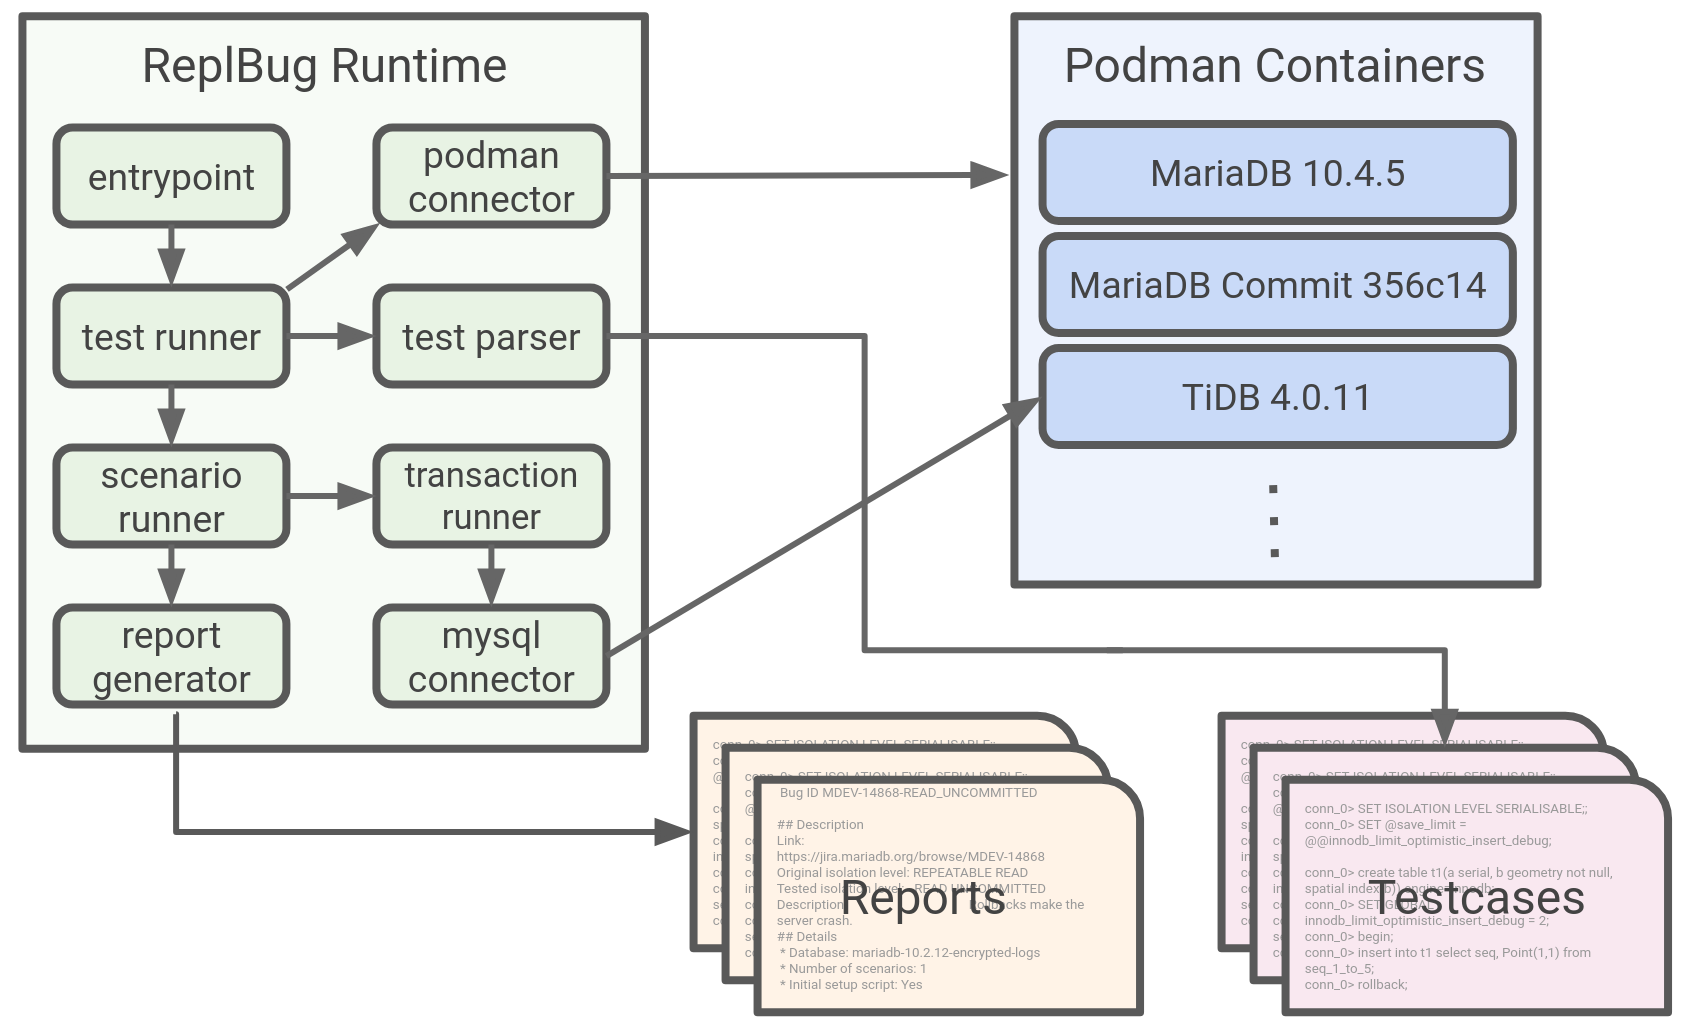
\includegraphics[width=\linewidth]{assets/replbug_design.png}
    \caption{Design of the \textit{ReplBug} testing framework}
    \label{fig:replb_design}
\end{figure}


The framework is modular, helping any future developer to easily extend it (for instance for adding support for new DBMSs). The main components in the bug testing pipeline (see Figure \ref{fig:replb_design}) are the following:

\begin{itemize}
    \item The \textit{podman connector}: This component handles the interaction with the \textit{Podman} engine, and is responsible for starting, stopping, downloading and managing containers running DBMS instances.
    \item The \textit{test parser}: This component handles the parsing of testcases, using a specific format, and is responsible for creating the internal representation of the testcases.
    \item The \textit{mysql connector}: This component handles the connection to a DBMS instance (running within a container), and is responsible for executing statements in order and extracting the results.
    \item The \textit{transaction runner}: This component handles the execution of all the statements in a transaction, and runs on different threads for concurrency.
    \item The \textit{scenario runner}: This component runs testcases under a specific configuration.
    \item The \textit{test runner}: This component orchestrates the execution of all required testcases under all specified configurations. 
\end{itemize}

\section{Custom DBMS Version}

Some bugs are specific to a certain version of a DBMS, which might not be available as pre-built binaries. For instance, versions with serious vulnerabilities are usually removed from official repositories, or intermediary versions tied to a specifig \textit{Git} commit are not released as binaries.

For the mentioned reasons, we consider the ability to built DBMSs from source essential. To simplify the process, we provide sample \textit{Dockerfile} templates, which can be used to test specific DMBS versions. A sample \textit{Dockerfile} for \textit{TiKV} can be seen in Figure \ref{fig:dockerfilesample}.
 
\begin{figure}
\begin{minted}[bgcolor=bg]{Dockerfile}
FROM golang:1.19-alpine AS builder

# Install git and other dependencies
RUN apk add --no-cache git make bash gcc wget binutils-gold \
    musl-dev curl tar

# Set the working directory inside the container and
# create necessary directories
RUN mkdir -p /go/src/github.com/pingcap
WORKDIR /go/src/github.com/pingcap

ARG TIDB_COMMIT=c9288d246c99073ff04304363dc7234d9caa5090

# Clone and build the TiDB repository
RUN git clone --depth 1 https://github.com/pingcap/tidb.git \
    && cd tidb \
    && git fetch --depth 1 origin "$TIDB_COMMIT" \
    && git checkout "$TIDB_COMMIT" \
    && make -j \
    && mv bin/tidb-server /usr/local/bin/tidb-server \
    && cd .. \
    && rm -rf tidb

EXPOSE 4000
WORKDIR /usr/local/bin
CMD ["./tidb-server", "-P", "4000"]    
\end{minted}
\caption{Sample \textit{Dockerfile} for building a specific version of \textit{TiDB}}
\label{fig:dockerfilesample}
\end{figure}

In our project, we provide \textit{Dockerfiles} for \textit{MySQL}, \textit{MariaDB} in release or debug mode, and \textit{TiDB} with or without \textit{TiKV}. Creating a new docker file only requires the \textit{Git} commit, and then running the \textit{build} command integrated into \textit{ReplBug}. 

\section{Testing Meta-Language}

For a given testcase, specifying the statements and their execution order on the DBMS is hard, due to multiple reasons:
\begin{itemize}
    \item Transactional and isolation bug PoCs usually need multiple concurent transactions, making a simple \textit{SQL} script insufficient.
    \item Some statements are expected to fail, which might lead to the termination of a standard script.
    \item The order of the statement execution (and sometimes the locking order) is important for the bug to manifest.
\end{itemize} 

To address these issues, the \textit{MySQL} development team created a testing framework which encodes testcases in a special format \cite{mysqltestrun}. Using this format, however, is cubersome, as we only need a small subset of the features, and using the \textit{MySQL} interpreter would make it hard to test other DBMSs. 

We thus create a small, custom scripting language on top of \textit{Python}, inspired by the way bug reporters describe their PoCs. In Figure \ref{fig:bug_metalanguage_sample}, we present a sample testcase for the bug \textit{MDEV-26642} in \textit{MariaDB 10.6.17}.

\begin{figure}
\begin{minted}[bgcolor=bg]{Python}
ORIGINAL_ISOLATION_LEVEL = DEFAULT_ISOLATION_LEVEL
BUG_ID = "MDEV-26642"
LINK = "https://jira.mariadb.org/browse/MDEV-26642"
DB_AND_VERSION = db_config.DatabaseTypeAndVersion(
    db_config.DatabaseType.MARIADB, "10.6.17"
)
SETUP_SQL_SCRIPT = """
create table t(a int, b int);
insert into t values (0, 0), (1, 1), (2, 2);
"""

DESCRIPTION = "The last select does not respect the update
                (a should always be 10)."


def get_scenarios(isolation_level: IsolationLevel):
    return [
        f"""
        conn_0> SET GLOBAL TRANSACTION ISOLATION LEVEL
                                {isolation_level.value};
        conn_0> begin;
        conn_0> select * from t;
        conn_1> begin;
        conn_1> update t set a = 10 where b = 1;
        conn_1> commit;
        conn_0> select * from t;
        conn_0> update t set a = 10 where true;
        conn_0> select * from t;
        conn_0> commit;
        """,
    ]
\end{minted}
\caption{Replication script for the bug \textit{MDEV-26642} in \textit{MariaDB 10.6.17}.} \label{fig:bug_metalanguage_sample}
\end{figure}

Each testcase provides the following information:
\begin{itemize}
    \item The \textit{DBMS} and version on which the bug was reported.
    \item The bug ID and a link to the bug report.
    \item The setup script, which is executed before the testcases. If the setup script is too long, it can be stored in a separate file.
    \item The description of the bug.
    \item The scenarios, which are the testcases that will be executed (one for each isolation level). Each scenario is a sequence of statements, executed in parallel by different connections.
\end{itemize}

For running a testcase, the tool provisions the required DBMS instance, executes the setup script (if present), and then runs the scenarios under all supported isolation levels. For each transaction a separate connection to the DBMS server is created. The results are then stored in a report, which can be further analysed.

\section{Usage}



\begin{figure}
    \centering
    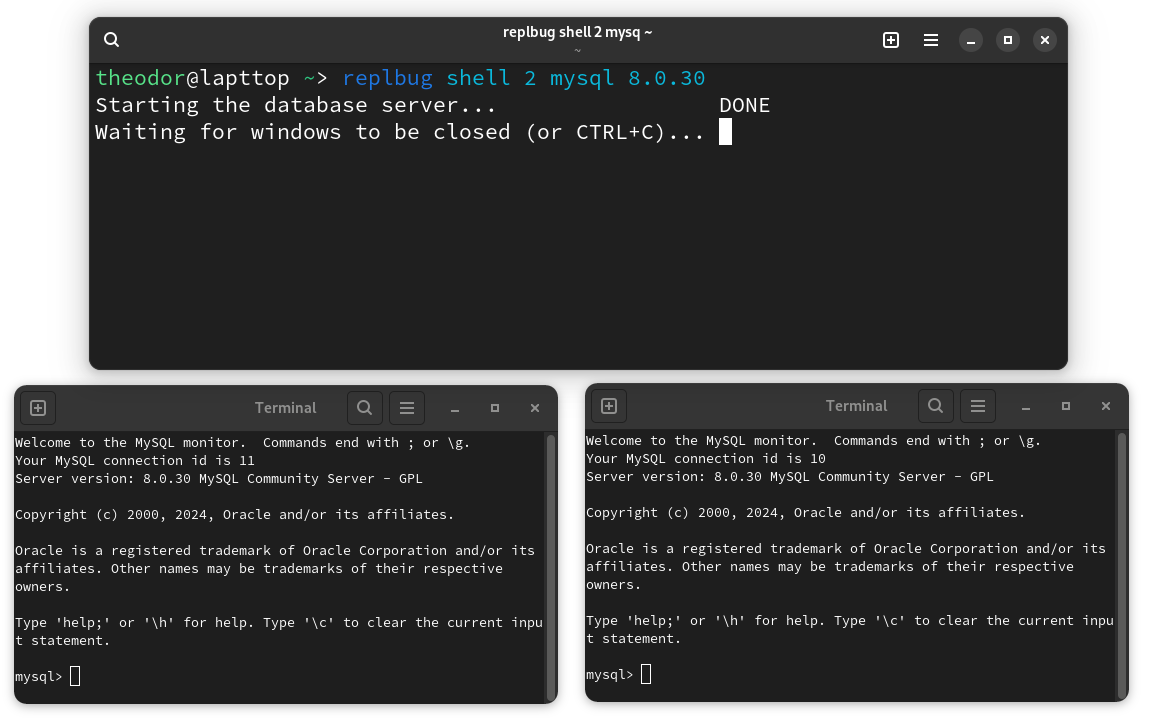
\includegraphics[width=\linewidth]{assets/replbug_shell.png}
    \caption{Using \textit{ReplBug} to start 2 \textit{MySQL v8.0.30} shells}
    \label{fig:replb_shell}
\end{figure}

\begin{figure}
    \centering
    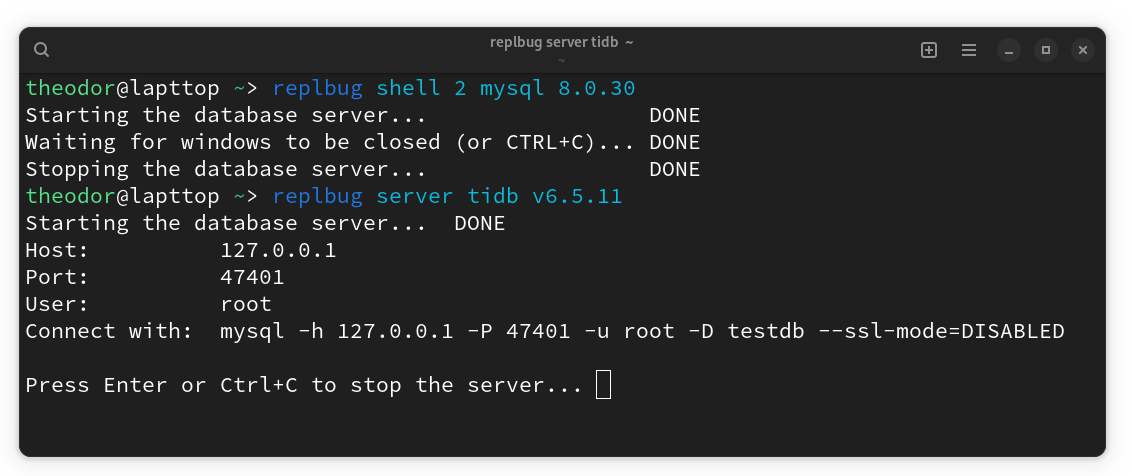
\includegraphics[width=\linewidth]{assets/replbug_server.png}
    \caption{Using \textit{ReplBug} to start a \textit{TiDB v6.5.11} server}
    \label{fig:repl_server}
\end{figure}

\begin{figure}
    \centering
    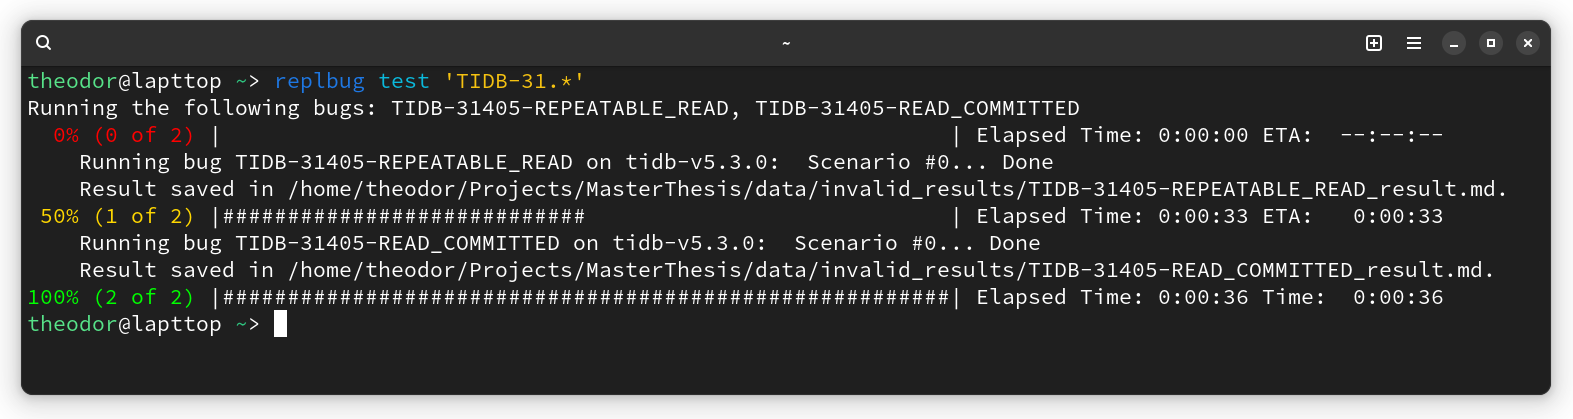
\includegraphics[width=\linewidth]{assets/replbug_test.png}
    \caption{Using \textit{ReplBug} to generate reports of some known bugs}
    \label{fig:repl_test}
\end{figure}


\begin{figure}
    \centering
    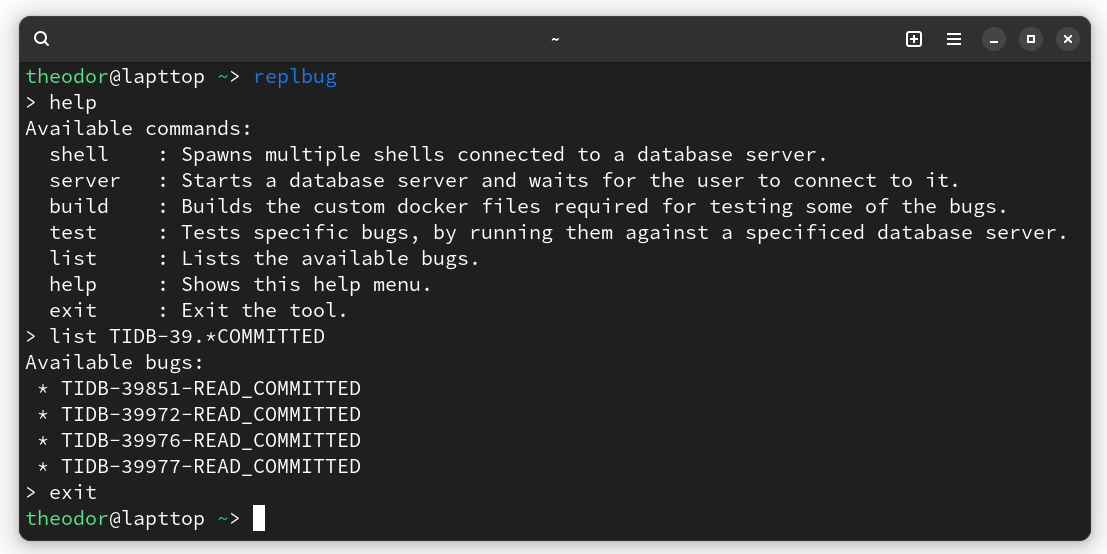
\includegraphics[width=\linewidth]{assets/replbug_interactive.png}
    \caption{Using \textit{ReplBug} in interactive mode}
    \label{fig:repl_interactive}
\end{figure}




The testing framework, called \textit{ReplBug} is invoked from the CLI. The main features it offers, exposed by the executable as subcommands are the following:
\begin{itemize}
    \item \textbf{\code{shell}} (See Figure \ref{fig:replb_shell}): Starts one or multiple \textit{MySQL}, \textit{MariaDB} or \textit{TiDB} shells, connected to a specific version of the DBMS. If the version is not present on the local machine, the tool will attempt to pull the image from Docker Hub.
    \item \textbf{\code{server}} (See Figure \ref{fig:repl_server}): Starts a specific version of the \textit{MySQL}, \textit{MariaDB} or \textit{TiDB} DBMS and provides the required details (host, port, user) for connecting to the server.
    \item \textbf{\code{test}} (See Figure \ref{fig:repl_test}): Runs the scenarios of some known bugs (which have to be written in a specific format prior), and automatically generates reports of the execution.
    \item \textbf{\code{list}}: Returns a list of the testcases available in the tool (optionally a \textit{regex} can be passed to filter the results).
\end{itemize}

The tool can be either used from the CLI by passing arguments, or in interactive mode, where the tool exposes a shell that can be used by the user  (see Figure \ref{fig:repl_interactive}).

\chapter{Replicating Transactional Bugs in MySQL, MariaDB and TiDB}

\section{Overview}

With the help of the \textit{ReplBug} testing framework, we were able to replicate \textit{MySQL}, \textit{MariaDB} and \textit{TiDB} transactional, logical and isolation bugs. We focus on transaction and isolation bugs, reported by DBMS testing papers \cite{cui2024understanding_ICSE2024, dou2023detecting_ICSE2023, cui2022differentially_ASE2022}. We then replicate the bugs on the same versions of the DBMSs, and verify which isolation levels are affected. The number of bugs taken from each paper can be seen in Figure \ref{fig:bugs_by_paper}.

\section{Replicated Bugs}


We try to replicate \textit{MySQL} and \textit{MariaDB} bugs on the $4$ isolation levels supported by the DBMSs (\textit{Read Uncommitted}, \textit{Read Committed}, \textit{Repeatable Read} and \textit{Serializable}). For \textit{TiDB}, we replicate the bugs on the $2$ isolation levels supported by the DBMS (\textit{Read Committed} and \textit{Serializable}).

\begin{figure}
    \centering
    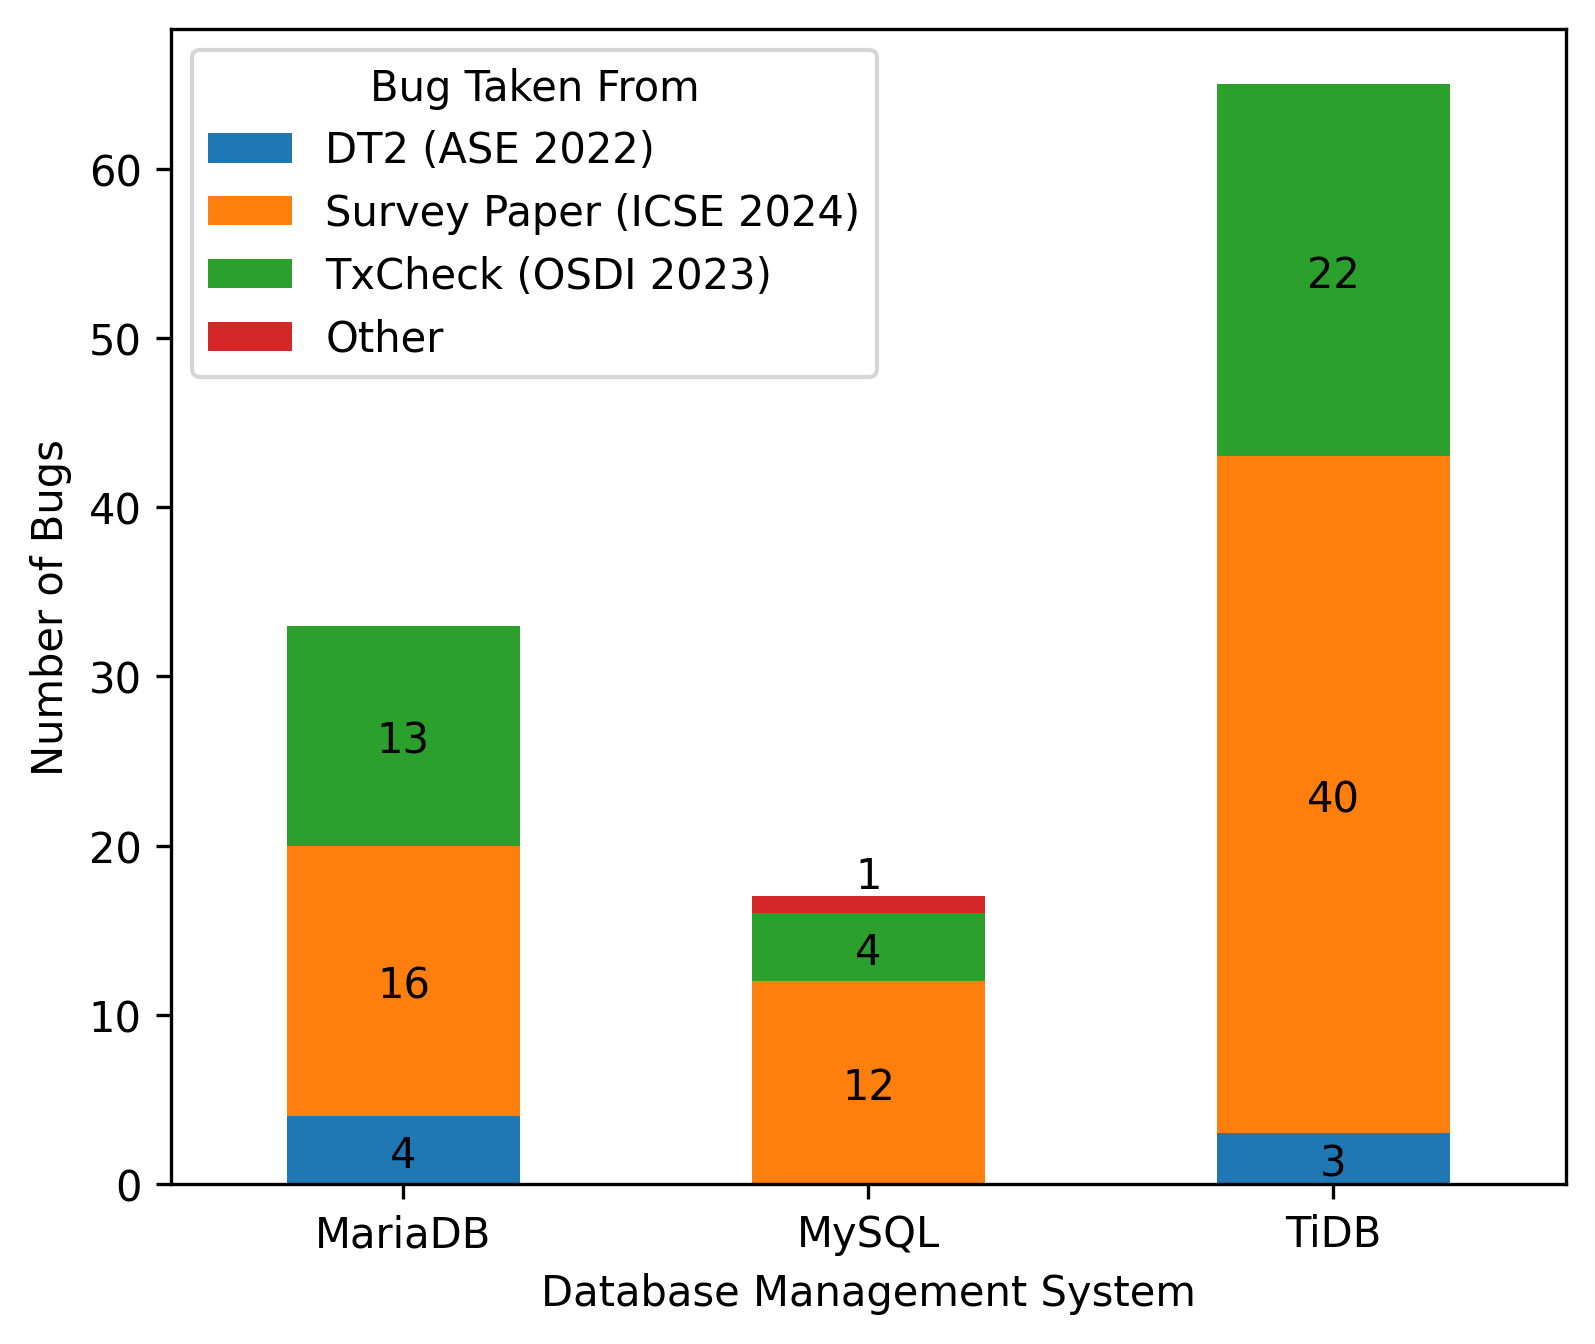
\includegraphics[width=0.8\linewidth]{assets/bug_replication_bugs_by_dbms_and_paper.png}
    \caption{Distribution of bugs by DBMS and reporting paper  \cite{cui2024understanding_ICSE2024, dou2023detecting_ICSE2023, cui2022differentially_ASE2022}.}
    \label{fig:bugs_by_paper}
\end{figure}

The methodology for replicating a bug is the following:
\begin{itemize}
    \item We search for the list of bugs reported by a paper, and filter the bugs that are transactional or isolation bugs (as reported by the paper), and manifest on one of the DBMSs we support (\textit{MySQL}, \textit{MariaDB} and \textit{TiDB}).
    \item We read the bug report in the DBMS's bug tracker, extract the version of the DBMS on which the bug was reported and a PoC.
    \item If the DBMS version is not available as a pre-built binary, we build the DBMS from source using the \textit{Dockerfile} templates provided by the \textit{ReplBug} tool.
    \item We write a testcase in the \textit{ReplBug} testing framework, using the meta-language described in the previous chapter.
    \item We run the testcase on the DBMS, under all supported isolation levels.
    \item We sometimes have to adjust the testcase, as some reports do not include the exact version of the DBMS, or the PoC is precise enough. 
\end{itemize}

Within this project, we successfully replicated $115$ bugs, out of which $33$ manifest on the \textit{MariaDB} DBMS, $17$ manifest on \textit{MySQL} and $65$ manifest on \textit{TiDB}. The distribution of the bugs by DBMS and reporting paper can be seen in Figure \ref{fig:interesting_bugs_by_paper}.

\section{Analysis}

We run the \textit{ReplBug} testing framework on the selected bugs, and we generate reports of their execution. We then read the reports, and analyse the output of the testcases. We then explore the corelation between the bugs and the isolation levels.

We find that $100$ bugs manifest on all isolation levels supported by the DBMS, and $15$ bugs only manifest on a subset of the isolation levels. In the reminder of this chapter, we refer to the bugs that manifest only on a subset of the isolation levels as \textit{interesting bugs}. In Figure \ref{fig:interesting_bugs_by_paper}, we present the distribution of the \textit{interesting bugs} by DBMS and reporting paper.

\begin{figure}
    \centering
    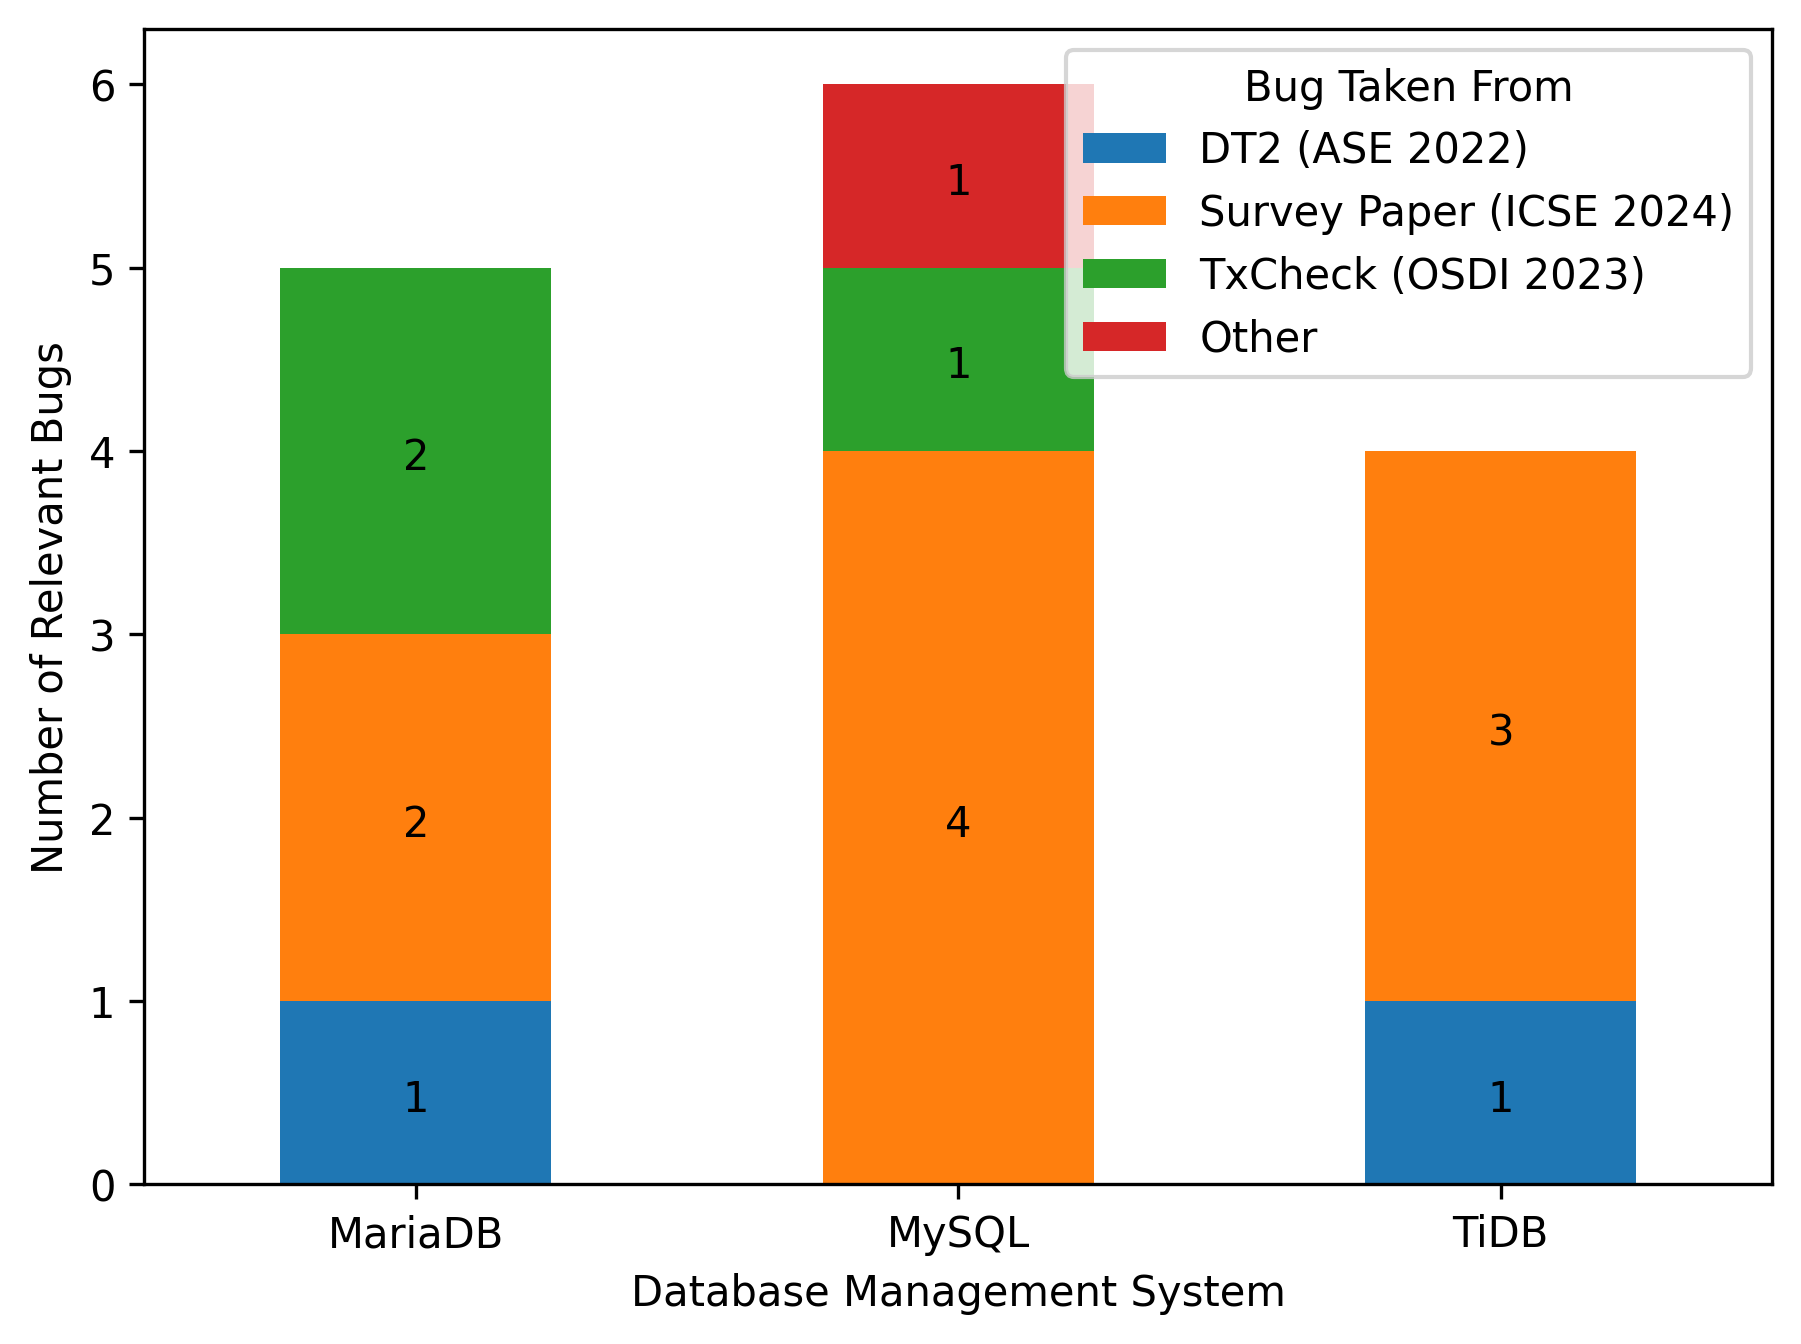
\includegraphics[width=0.8\linewidth]{assets/bug_replication_interesting_bugs_by_dbms_and_paper.png}
    \caption{Relevant bugs by DBMS and reporting paper  \cite{cui2024understanding_ICSE2024, dou2023detecting_ICSE2023, cui2022differentially_ASE2022}.}
    \label{fig:interesting_bugs_by_paper}
\end{figure}


We then explore the isolation levels under which the \textit{interesting bugs}, manifest. We find that:
\begin{itemize}
\item 5 bugs manifest under \textit{Read Committed} and \textit{Repeatable Read}.
\item 4 bugs manifest under \textit{Repeatable Read}.
\item 2 bugs manifest under \textit{Read Uncommitted} and \textit{Read Committed}.
\item 2 bugs manifest under \textit{Read Committed}.
\item One bug manifests under \textit{Serializable}.
\item One bug manifests under \textit{Repeatable Read} and \textit{Serializable}.
\end{itemize}

The findings are illustrated in Figure \ref{fig:interesting_bugs_by_isolation_lvl}. The main limitation of this analysis is that the number of \textit{intersting bugs} is small, making the results not statistically significant. Additionally, our approach only allows us to verify if a bug is triggered by a specific PoC, and not to explore the root cause of the bug, which could in theory be triggered by other PoCs under different isolation levels.

\begin{figure}
    \centering
    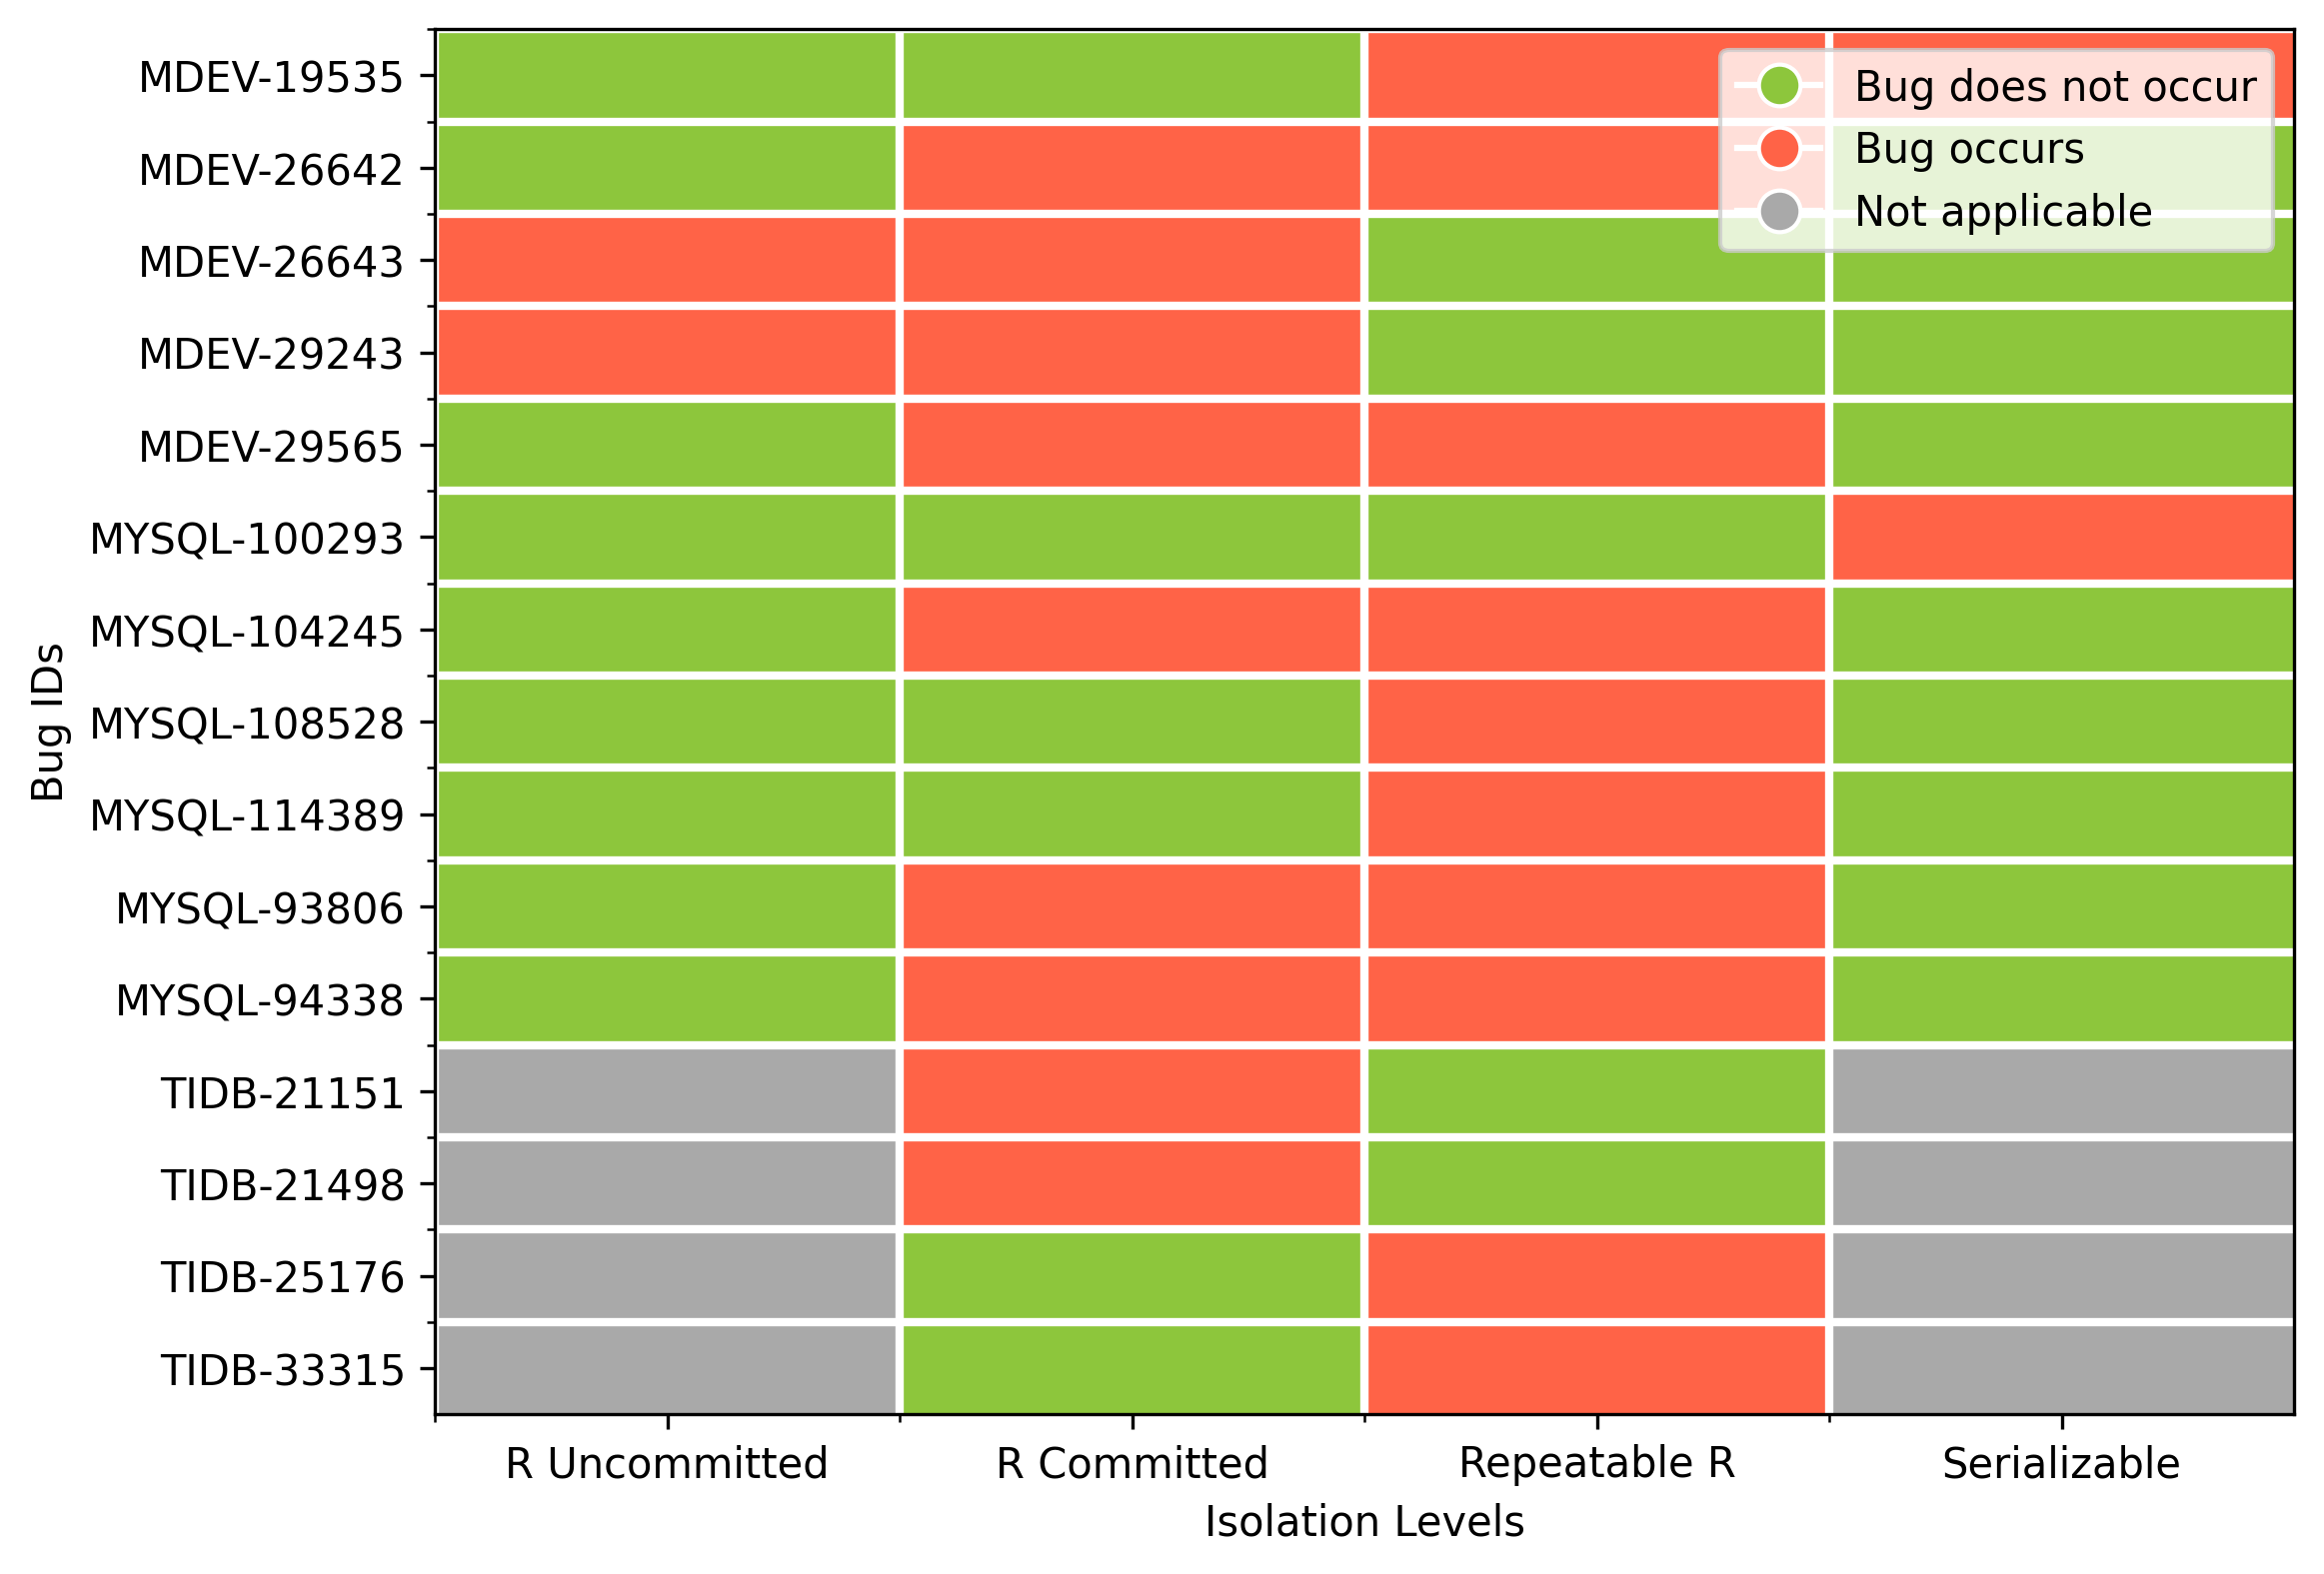
\includegraphics[width=0.9\linewidth]{assets/bug_replication_interesting_bugs_by_isolation_lvl.png}
    \caption{Relevant bugs by isolation levels.}
    \label{fig:interesting_bugs_by_isolation_lvl}
\end{figure}

\section{Interesting Bugs}

We present a brief overview of the \textit{interesting bugs}, and provide a plausible explanation for their behaviour, where possible. The bugs are presented in the order of the number of isolation levels under which they manifest.

\subsection*{Bug MDEV-19535}

This bug is replicated on \textit{MariaDB 10.4.5}, and manifests under \textit{Repeatable Read} and {Serializable}.

For compatibility, \textit{MariaDB} provides an \code{sql\_mode} variable, which can be used to mimic the behaviour of other DBMSs.

When the \code{sql\_mode} is set to \code{ORACLE}, \textit{MariaDB} ommits to add exclusive locks when running an \textit{SELECT FOR UPDATE} statement. This leads to incorrect hehaviour when running \textit{SELECT FOR UPDATE} statements under \textit{Repeatable Read} and \textit{Serializable} isolation levels, as reads are no longer guaranteed to be repeatable.

\subsection*{Bug MDEV-26642}


This bug is replicated on \textit{MariaDB 10.6.17}, and manifests under \textit{Read Committed} and \textit{Repeatable Read}. The bug was fixed by a PR in version \textit{$10.6.18$}, and was marked as affecting \textit{MySQL} too.


The bug affects concurent modifications of the same table: if a transaction updates a row of the table, and another transaction updates the entire table, the second transaction does not see its own modifications. The main part of the PoC can be seen in Figure \ref{fig:MDEV-26642}.


\begin{figure}
\begin{minted}[bgcolor=bg]{SQL}
conn_0> begin;
conn_0> select * from t;        -- [(0, 0), (1, 1), (2, 2)]

conn_1> begin;
conn_1> update t set a = 10 where b = 1;
conn_1> commit;

conn_0> select * from t;        -- [(0, 0), (1, 1), (2, 2)]
conn_0> update t set a = 10 where true;
conn_0> select * from t;        -- [(10, 0), (1, 1), (10, 2)]
conn_0> commit;
\end{minted}
\caption{PoC for the bug \textit{MDEV-26642}.} \label{fig:MDEV-26642}
\end{figure}

The bug is caused by a design issue of \textit{InnoDB}, the storage engine used by both \textit{MariaDB} and \textit{MySQL}.

The bug is due to the inability of \textit{InnoDB} to detect \textit{write-write} conflicts. Under \textit{Read Committed} and \textit{Repeatable Read}, \textit{InnoDB} creates a read view at the start of a statement / transaction, used for knowing which records should be visible, but does not handle overwriten records properly. 

The \textit{Read Uncommitted} isolation level always displays the latest state of the table, and \textit{Serializable} will lock the accessed records first, so the bug does not manifest under these isolation levels.

\subsection*{Bug MDEV-26643}


This bug is replicated on \textit{MariaDB 10.5.12}, and manifests under \textit{Read Uncommitted} and \textit{Read Committed}. The bug was fixed by a PR.The PoC is very similar to \textit{MDEV-26642}, and can be seen in Figure \ref{fig:MDEV-26643}.


\begin{figure}
\begin{minted}[bgcolor=bg]{SQL}
conn_0> insert into t values(null, 1), (2, 2),
                    (null, null), (null, 3), (4, null);
conn_0> begin;
conn_0> update t set a = 10 where 1;
conn_1> begin;
conn_1> update t set b = 20 where a;
conn_0> commit;
conn_1> commit;
conn_2> select * from t; 
        -- [(10, 1), (10, 20), (10, 20), (10, 20), (10, 20)]
\end{minted}
\caption{PoC for the bug \textit{MDEV-26642}.} \label{fig:MDEV-26643}
\end{figure}

The bug is caused by an improperly used semi-consistent read, where \textit{Read Uncommitted} and \textit{Read Committed} transactions are sometimes not updated with the latest changes.

\subsection*{Bug MDEV-29243}

This bug is replicated on \textit{MariaDB 10.8.3}, and manifests under \textit{Read Uncommitted} and \textit{Read Committed}, by causing a crash of the DBMS server.

The root cause of the bug is an incorrect and redundant check of the data retrival status in \textit{InnoDB}, which leads to potential assertion failures. The bug was fixed by erasing the redundant check.

\subsection*{Bug MDEV-29565}

This bug is replicated on \textit{MariaDB 10.8.3}, and manifests under \textit{Read Committed} and \textit{Repeatable Read}.

While confirmed as intented behaviour, this is caused by an poorly documented feature of \textit{InnoDB}, which allows changes made by other transactions to be visible in the current one if changes are made to the same records \cite{mysqlconsistentread}. The PoC is simplified in Figure \ref{fig:MDEV-29565}.

\begin{figure}
\begin{minted}[bgcolor=bg]{SQL}
conn_1> START TRANSACTION;
conn_1> update t set a = 162;
conn_0> START TRANSACTION;
conn_1> COMMIT;
conn_0> select * from t where <CONDITION>; -- returns 1 record
conn_0> update t set a = 63 where <CONDITION>;
conn_0> select * from t where a = 63;      -- returns 2 records
conn_0> COMMIT;
\end{minted}
\caption{Simplification of the PoC for the bug \textit{MDEV-29565}.} \label{fig:MDEV-29565}
\end{figure}


\subsection*{Bug MYSQL-100293}

This bug is replicated on \textit{MySQL 5.7.31}, and manifests under \textit{Serializable}.

When the \code{innobase\_query\_caching\_of\_table\_permitted} flag is set to \code{true} (by passing \code{--query-cache-type=1} as an argument to the server), \textit{Serialisable} transactions are not blocked when using the cache, which causes some missing locks.

The bug was fixed by properly handling \code{--query-cache-type=1} when the transaction isolation level is \textit{Serializable}.

\subsection*{Bug MYSQL-104245}


This bug is replicated on \textit{MySQL 8.0.23}, and manifests under \textit{Read Committed} and \textit{Repeatable Read}.

Wen inserting rows with the same primary key multiple times (using the \code{INSERT IGNORE} statement), row locks are duplicated. Using \code{REPLACE INTO} is even worse, and adds many row locks (we believe the number of added locks is the number of matched records times the number of inserted records).

The bug only manifests on \textit{Read Committed} and \textit{Repeatable Read}, as \textit{Serializable} has a different locking mechanism, and \textit{Read Uncommitted} does not lock the records at all.

This bug dramatically increases latency, but does not cause deadlocks or crashes, as all the redundant row locks are identical. The bug is not present in \textit{MySQL 8.0} or later, so it was not fixed.

\subsection*{Bug MYSQL-108528}

This bug is replicated on \textit{MySQL 5.7.34}, and manifests under \textit{Repeatable Read}.

The bug is marked as verified, but we strongly consider the PoC actually works as intented. The PoC is simplified in Figure \ref{fig:MYSQL-108528}.

In the PoC, one transaction updates a table and commits. Another concurent transaction does not see the changes made by the first transaction, however those changes become visible when the second transaction tried to update a table. This behaviour is similar to the behaviour of \textit{MDEV-29565}, and we consider it is due to the same poorly-documented feature \cite{mysqlconsistentread}.


\begin{figure}
\begin{minted}[bgcolor=bg]{SQL}
    conn_1> START TRANSACTION;
    conn_0> START TRANSACTION;
    conn_0> select * from t_rpjlsd;         -- Create snapshot.

    conn_1> update t_g6ckkb set wkey = 162; -- Update the table.
    conn_1> COMMIT;                         -- Commit.

    conn_0> select * from t_rpjlsd where
                t_rpjlsd.c_pfd8ab <= (
                    select min(wkey)
                    from t_g6ckkb
                );                          -- Affects 1 row.
    conn_0> update t_rpjlsd set wkey = 63 where
                t_rpjlsd.c_pfd8ab <= (
                    select min(wkey)
                    from t_g6ckkb
                );                          -- Affects 2 rows.
\end{minted}
\caption{Simplification of the PoC for the bug \textit{MYSQL-108528}.} \label{fig:MYSQL-108528}
\end{figure}



\subsection*{Bug MYSQL-114389}

This bug is replicated on \textit{MySQL 8.0.12}, and manifests under \textit{Repeatable Read}. The bug is still present in the latest version of \textit{MySQL} (version \textit{9.1.0}). It was closed as \textit{duplicate}, but the original bug is still open.

As the bug is still open, we do not know the root cause of the bug, whose PoC can be seen in Figure \ref{fig:MYSQL-114389}.

\begin{figure}
\begin{minted}[bgcolor=bg]{SQL}
conn_0> BEGIN;

conn_1> BEGIN;                          
conn_1> UPDATE t SET b = 222, c = 333;   -- Update the table.
conn_1> COMMIT;                         

conn_2> BEGIN;
conn_2> SELECT pkId, b, c FROM t;        -- Create snapshot.

conn_0> UPDATE t SET a = 40 WHERE a = 44;
conn_0> COMMIT;

conn_2> UPDATE t SET b = 888, c = 999;   -- Update the table.
conn_2> SELECT pkId, b, c FROM t where   -- Should be empty but
          b = 854 or c = 333 order by b; -- returns a row.

\end{minted}
\caption{PoC for the bug \textit{MYSQL-114389}.} \label{fig:MYSQL-114389}
\end{figure}


\subsection*{Bug MYSQL-93806}

This bug is replicated on \textit{MySQL 8.0.12}, and manifests under \textit{Read Committed} and \textit{Repeatable Read}. The bug was fixed as part of the \textit{MySQL 8.0.16} release.

The bug is caused by a misshandling of the \code{INSERT ... ON DUPLICATE KEY} statement. When a record with a conflicting primary key is inserted, the key should be changed and a row lock created. However, under \textit{Read Committed} and \textit{Repeatable Read}, a range lock is created instead. The PoC is simplified in Figure \ref{fig:MYSQL-93806}.

\begin{figure}
\begin{minted}[bgcolor=bg]{SQL}
conn_0> create table t(id int primary key, a int)engine=innodb;
conn_0> insert into t values(1,1),(5,5);

conn_0> SET GLOBAL TRANSACTION ISOLATION LEVEL REPEATBLE READ;
conn_0> begin;
conn_0> insert into t values(5,5) ON DUPLICATE
            KEY UPDATE a=a+1; -- Creates a range lock instead
                              -- of a row lock.

conn_1> begin;
conn_1> insert into t values(4, 4); -- Is needlessly blocked by
                                    -- the range lock.
\end{minted}
\caption{Simplification of the PoC for the bug \textit{MYSQL-93806}.} \label{fig:MYSQL-93806}
\end{figure}


\subsection*{Bug MYSQL-94338}

This bug is replicated on \textit{MySQL 5.7.25}, and manifests under \textit{Read Committed} and \textit{Repeatable Read}. The bug is not present in \textit{MySQL 8.0} or later, so it was not fixed.

The bug manifests by causing diry-reads when inserting multiple rows on one transaction, and performing a complex query on another transaction. The PoC is simplified in Figure \ref{fig:MYSQL-94338}. We do not know the root cause of the bug, as no bug fix was made available.

\begin{figure}
\begin{minted}[bgcolor=bg]{SQL}

        conn_0> BEGIN;
        conn_1> BEGIN;

        conn_1> INSERT INTO t VALUES
                (1,40,'B',10,1),
                (1,41,'B',10,1),
                ...
                (1,40,'C',16,1),
                (1,42,'C',16,1);

        conn_0> SELECT * FROM t1
                WHERE <<CON`DITION>>; -- Dirty read.;
\end{minted}
\caption{Simplification of the PoC for the bug \textit{MYSQL-94338}.} \label{fig:MYSQL-94338}
\end{figure}

\subsection*{Bug TIDB-21151}

This bug is replicated on \textit{TiDB v4.0.8} when using the \textit{TiKV} key-value store, and manifests under \textit{Read Committed}. The bug was closed by a PR pushed to the \code{master} branch on \textit{2020-11-24}.

The bug occurs because the \code{USE\_INDEX\_MERGE} feature does not refresh the current timestamp of the transaction, causing the transaction to potentially miss the latest committed writes. While this is correct to \textit{REPETABLE READ} transactions, \textit{READ COMMITTED} transactions are expected to see committed changes. A simplified PoC can be seen in Figure \ref{fig:TIDB-21151}. 

The bug fix correctly updates the timestamp used by transactions when running under \textit{READ COMMITTED}, by invoking the \code{refreshForUpdateTSForRC} function when required.

\begin{figure}
\begin{minted}[bgcolor=bg]{SQL}
conn_0> BEGIN;

-- Update the table, after transaction 0 started.
conn_1> BEGIN;
conn_1> update t set value = 11 where id = 2;
conn_1> COMMIT;

conn_0> select /*+ NO_INDEX_MERGE() */ *
            from t where a > 3 or b > 3;   -- Ok.

conn_0> select /*+ USE_INDEX_MERGE(t, ia, ib) */ *
            from t where a > 3 or b > 3;   -- Misses the update.
\end{minted}
\caption{Simplification of the PoC for the bug \textit{TIDB-21151}.} \label{fig:TIDB-21151}
\end{figure}

\subsection*{Bug TIDB-21498}

This bug is replicated on \textit{TiDB}, on the custom commit \code{3a32bd2d} using the \textit{TiKV} key-value store, and manifests under \textit{Read Committed}. The bug was closed by a PR pushed to the \code{master} branch on \textit{2021-01-12}.

The bug occurs because of missing consistency checks which allow one concurent transaction to perform DDL (Data Definition Language) operations on a table (like inserting / deleting columns or deleting indexes), while another transaction is reading from the same table. The PoC is simplified in Figure \ref{fig:TIDB-21498}.

\begin{figure}
\begin{minted}[bgcolor=bg]{SQL}
conn_0> begin;

conn_1> alter table t drop index iv;
conn_1> update t set v = 11 where id = 1;

conn_0> select * from t where v = 10; -- Returns [1, 10].
conn_0> select * from t where id = 1; -- Returns [1, 11].
\end{minted}
\caption{Simplification of the PoC for the bug \textit{TIDB-21498}.} \label{fig:TIDB-21498}
\end{figure}

\subsection*{Bug TIDB-25176}

This bug was reported on a specific commit of the \code{master} branch, is replicated on \textit{TiDB 4.0.7} when using the \textit{TiKV} key-value store, and manifests under \textit{Repeatable Read}. The bug is still open as of \textit{November 2024}.

The bug is due to the usage of the \code{tidb\_snapshot} system variable, which sets the timestamp delimiting the visibility of the records \cite{tidbsnapshot}. 

Under \textit{Repetable Read}, setting this timestamp and the performing a \code{SELECT} statement breaks the isolation level guarantees. The PoC is simplified in Figure \ref{fig:TIDB-25176}.

\begin{figure}
\begin{minted}[bgcolor=bg]{SQL}
conn_0> begin;                              -- Start txn.
    
conn_1> update test.ttt set a=2 where id=1; -- Update records.

conn_0> set @@tidb_snapshot=TIMESTAMP(NOW());

conn_0> select a from test.ttt where id=1;            -- [(1)].
conn_0> select a from test.ttt where id=1 for update; -- [(2)].
conn_0> select a from test.ttt where id=1;            -- [(2)].
\end{minted}
\caption{Simplification of the PoC for the bug \textit{TIDB-25176}.} \label{fig:TIDB-25176}
\end{figure}

\subsection*{Bug TIDB-33315}

This bug is replicated on \textit{TiDB 5.4.0} when using the \textit{TiKV} key-value store, and manifests under \textit{Repeatable Read}. 

The bug is caused by the mismatch of rows created by concurent transactions: if a transaction performs a statement matching an entire table while another transaction holds an exclusive lock on the table, the first transaction will see an inconsistent state. The PoC is simplified in Figure \ref{fig:TIDB-33315}.

\begin{figure}
\begin{minted}[bgcolor=bg]{SQL}
conn_0> BEGIN PESSIMISTIC;
conn_0> UPDATE t SET c1=2, c2=2;

conn_1> BEGIN PESSIMISTIC;
conn_1> DELETE FROM t;     -- Delete all records.

conn_0> COMMIT;            -- First transaction commits.

conn_1> SELECT * FROM t;   -- Returns one row.
conn_1> COMMIT;
\end{minted}
\caption{Simplification of the PoC for the bug \textit{TIDB-33315}.} \label{fig:TIDB-33315}
\end{figure}


\section{Conclusion}

In this chapter, we present an analysis of a few isolation bugs we consider \textit{interesting}, as they manifest under a subset of the isolation levels supported by the DBMSs. We provide a brief overview of the bugs, and a plausible explanation for their behaviour.

We find that the bugs are caused by a variety of reasons, from design issues of the storage engine to poorly documented features of the DBMSs. We also find that some bugs are quickly fixed, while others are left unfixed until they \textit{fix themselves}, i.e. they are no longer present in the latest versions of the DBMSs.

The main cause of bugs is the improper handling of locking and MVCC (Multi-Version Concurrency Control) mechanisms, which are the core of the transactional guarantees provided by the DBMSs, as \textit{MySQL}, \textit{MariaDB} and \textit{TiDB} define their isolation levels based on locking behaviour and transaction visibility \cite{mysqlisolationlevels,mariadbtransactions,tidbisolationlevels}.

\chapter{Detecting Isolation Bugs in DBMSs via Dependency Graphs Construction}

\section{Introduction and Motivation}

As discussed in the previous chapter, and in various other works \cite{jiang2023detecting,cui2024understanding_ICSE2024,dou2023detecting_ICSE2023,clark2024validating,cui2022differentially_ASE2022}, isolation bugs are a prevalent problem in DBMSs, due to the inherent trade-off between performance (under the form of concurrency) and isolation.

Modern database systems usually express isolation guarantees under a \textit{locking behavior}, which is a set of rules dictating how tables and rows are locked during transactions. However, due to the sheer complexity of modern DBMSs, ensuring a correct locking behavior is challenging, due to a combination of factors such as:

\begin{itemize}
    \item DBMS systems are complex, with multiple components interacting with each other, such as the query planner, the storage engine, the transaction manager, etc. A bug in any of these components can lead to an isolation bug.
    \item The performance of DBMSs is subject to the law of diminishing returns, requiring more and more complex optimizations to achieve smaller and smaller performance gains. This makes it more likely for bugs to be introduced.
    \item Higher concurrency leads to better performance, thus making a reduction in the number of locks desirable. However, this also makes it more likely for isolation bugs to occur.
\end{itemize}

As \textit{isolation bugs} are not necessarily \textit{logic bugs}, i.e. not bugs in the traditional sense but rather a violation of the isolation guarantees, hunting them with standard bug-finding techniques is challenging:

\begin{itemize}
    \item Testing high concurrency workloads, required for capturing edge cases where isolation bugs occur, is hard to achieve due to an exponential growth in the number of possible states.
    \item DBMSs are not fully compatible with each others, and concurrent workloads are inherently non-deterministic, making it hard to check for bugs by exploring differences between DBMSs.
    \item Semi-automatic techniques such as \textit{fuzzing} require an \textit{oracle} to determine if the output is correct, which is hard to achieve in the case of isolation bugs.
\end{itemize}

Current techniques avoid these problems by using a white-box testing approach \cite{clark2024validating}, using the database system itself as a testing oracle \cite{jiang2023detecting}, or running workloads on multiple DBMSs to check for disparities \cite{cui2022differentially_ASE2022}.

Following our work on the bug replication testbed, we explore potential next steps and decide to focus on \textit{TxCheck}, a database fuzzer, for several reasons:

\begin{itemize}
    \item \textit{TxCheck} is developed at ETH Zürich, making it a natural choice for in-depth research.
    \item It has successfully identified an impressive $56$ bugs in \textit{MariaDB}, \textit{MySQL}, and \textit{TiDB}, some of which we analyzed using our bug testbed.
    \item \textit{TxCheck} was released last year (2023), making it highly relevant.
\end{itemize}

In this chapter, we introduce our work on enhancing a novel bug-finding technique that leverages Direct Serialization Graphs (DSG) introduced by Adya, A. \cite{adya1999weak} and SQL-level instrumentation introduced by Jiang, Z. \cite{jiang2023detecting}. Our approach builds upon and modifies the method used by Jiang, Z. Additionally, we implement a tool based on our technique within the \textit{TxCheck} fuzzer, which we adapt to meet our requirements.


\section{Database Model Used}

For testing the correct behavior of database systems, we need well-defined specifications we can test against. While some techniques rely on the DBMSs themselves for self-validating or cross validating results \cite{cui2022differentially_ASE2022}, other bug-finding techniques express DBMS isolation bugs as violated constraints in the Direct Serialization Graph (DSG) built following Adya's data model \cite{jiang2023detecting,clark2024validating}, directed labeled graphs in which nodes are transactions and directed edges are dependencies.

In particular, \textit{TxCheck}, which this project builds on, uses a mixture of both methods:
\begin{itemize}
    \item Using \textit{SQL instrumentation}, \textit{TxCheck} extracts a super-graph of the DSG. However, the dependency checking technique used is not perfect, and can create sporadic dependencies.
    \item Using the DSG, \textit{TxCheck} creates and executes an equivalent execution trace using a single transaction on the same DBMS, which is used as an oracle for comparing the results.
\end{itemize}

In this work, we rely on the Direct Serialization Graph (DSG) data model introduced by Adya, A. \cite{adya1999weak}, and on the SQL-level instrumentation technique introduced by Jiang, Z. \cite{jiang2023detecting}.

\section{Contributions}

Our two main contributions are:

\begin{itemize}
    \item We build on the theory behind the DSG extraction used in \textit{TxCheck}, for allowing for a complete and sound extraction of all the DSG dependencies, by leveraging the \textit{SQL instrumentation} technique \textit{TxCheck} introduced. Our approach allows for an accurate extraction of the DSG edges, which avoids the sporadic dependencies created by the original technique, and allows for a more accurate detection of isolation bugs.
    \item We implement the changes in the \textit{TxCheck} project, giving \textit{TxCheck} the ability to extract the DSG edges accurately.
\end{itemize}


\section{Background on DSG Dependencies}

Throughout this work, we heavily reuse the definitions and notations introduced by Adya, A. \cite{adya1999weak}. The most important definitions are the ones regarding the dependencies between transactions, which we outline below.

\begin{definition}
    \label{def:overwriting}
    \textbf{Overwriting a Predicate}: $T_j$ overwrites an operation $r_i(P: Vset(P))$ or $w_i(P: Vset(P))$ if:
    \begin{itemize}
        \item $T_j$ installs a version $x_j$ for some object $x$.
        \item The version $x_k$ of $x$ present in $Vset(P)$ is an earlier version than $x_j$.
        \item $x_j$ matches the predicate $P$ and $x_k$ does not, or vice versa.
    \end{itemize}  
\end{definition}

\begin{definition}
    \textbf{Directly Item-Read-Depends}: $T_j$ \textit{directly item-read-depends} on $T_i$ if $T_j$ reads an some object version installed by $T_i$.
\end{definition}

\begin{definition}
    \textbf{Directly Predicate-Read-Depends}: $T_j$ \textit{directly predicate-read-depends} on $T_i$ if $T_j$ performs a read operation $r_j(P: Vset(P))$ and $T_i$ installs $x_i$ such that $x_i \in Vset(P)$.
\end{definition}

\begin{definition}
    \textbf{Directly Read-Depends}: $T_i$ \textit{directly read-depends} on $T_j$ if $T_i$ directly item-read-depends or directly predicate-read-depends on $T_j$.
\end{definition}

\begin{definition}
    \textbf{Directly Item-Anti-Depends}: $T_j$ \textit{directly item-anti-depends} on $T_i$ if $T_i$ reads some object version $x_k$ and $T_j$ installs a later version $x_j$.
\end{definition}

\begin{definition}
    \textbf{Directly Predicate-Anti-Depends}: $T_j$ \textit{directly predicate-anti-depends} on $T_i$ if $T_j$ overwrites the predicate of an operation $r_i(P: Vset(P))$. %  or $w_i(P: Vset(P))$.
\end{definition}

\begin{definition}
    \textbf{Directly Anti-Depends}: $T_i$ \textit{directly anti-depends} on $T_j$ if $T_i$ directly item-anti-depends or directly predicate-anti-depends on $T_j$.
\end{definition}

\begin{definition}
    \textbf{Directly Item-Write-Depends}: $T_j$ \textit{directly item-write-depends} on $T_i$ if $T_i$ installs a version $x_i$ and $T_j$ installs the next version $x_j$.
\end{definition}

\begin{definition}
    \textbf{Directly Predicate-Write-Depends}: $T_j$ \textit{directly predicate-write-depends} on $T_i$ if:
    \begin{itemize}
        \item $T_j$ overwrites an operation $w_i(P: Vset(P))$, or
        \item $T_j$ executes an operation $w_j(P: Vset(P))$ and $T_i$ installs some version $x_i \in Vset(P)$.
    \end{itemize}
\end{definition}

\begin{definition}
    \textbf{Directly Write-Depends}: $T_i$ \textit{directly write-depends} on $T_j$ if $T_i$ directly item-write-depends or directly predicate-write-depends on $T_j$.
\end{definition}

The steps for building the DSGs given an ordered sequence of statements (each belonging to a possibly different transaction) are as follows:
\begin{enumerate}
    \item Run the statements sequentially, saving the versions of the objects at each step.
    \item Extract the \textit{Direct Read Dependencies}, \textit{Direct Write Dependencies} and \textit{Direct Anti-Dependencies} between transactions.
    \item Build the DSGs using the extracted dependencies.
\end{enumerate}

The second step is the hardest, due to the inherent lack of information a DBMS provides about the internal state of the system. This is where SQL-level instrumentation comes in.

\section{SQL-level Instrumentation}

\subsection{Intuition Behind SQL-level Instrumentation}

The most straight-forward way to extract DSG dependencies is to modify the source code of DBMSs, exposing the internal state of the system. This allows for a relatively simple extraction of dependencies, as the injected code has access to all of the instruction scheduling, existing locks, state of the key-value store, etc. This is how Clark, J. et al. extract the DSGs in their work \cite{clark2024validating}.

A less intrusive approach, which considers the DBMS as a black box (thus being easily ported across different systems), is to use SQL-level instrumentation, a technique pioneered by Jiang, Z., which consists of systematically exposing the internal state of the DBMS by injecting \textit{SELECT} statements in the SQL queries \cite{jiang2023detecting}.

The informal intuition behind SQL-level instrumentation is that we want to know the current state of the database, but lack the white-box access to the DBMS internals. As we can only query the database, we infer the dependencies by injecting \textit{SELECT} statements in test cases. We instrument the SQL queries by adding instrumentation code right before and right after each original SQL statement.

A few challenging parts are:

\begin{itemize}
    \item Ensuring the instrumentation code is not interrupted by locking or other operations. This is addressed by re-ordering statements in the test case, and erasing them if no viable scheduling order can be found.
    \item Ensuring that every table of the database stores versioning information for each object, required for understanding the view a statement has access to. This is addressed by adding a \textit{version} column to each table.
    \item Concurrency issues, such as the non-deterministic locking and unlocking behavior of transactions. This is addressed by spacing out the statements temporally, and ensuring that no transaction locking takes place.
\end{itemize}


\subsection{Instrumentation Statements}

We instrument SQL statements by encapsulating them with instrumentation placed before and after statements, which expose the transaction's view of the database. As we built on top of \textit{TxCheck}, the instrumentation we use is very similar to the original one, with the addition of $3$ new instrumentation types. The instrumentation types we use are:

\begin{itemize}
    \item \textbf{Before Write Read (BWR)}: Before a write operation, a \textit{SELECT} statement is added to read the version of overwritten objects.
    \item \textbf{After Write Read (AWR)}: After a write operation, a \textit{SELECT} statement is added to read the new version of the overwritten objects.
    \item \textbf{Version Set Read (VSR)}: Before reads and predicated statements, a \textit{SELECT} statement is added to read the version set of all objects in the used tables.
    \item \textbf{Before Predicate Match (BPM)}: Before a write operation, a \textit{SELECT} statement is added for each predicate that appears in the test case, to read the objects and versions that match the predicate.
    \item \textbf{After Predicate Match (APM)}: Similar to the \textit{Before Predicate Match}, but is inserted after the write operation.
    \item \textbf{Predicate Match (PM)}: Before an operation that contains a predicate, a \textit{SELECT} statement reading the objects and versions that match the predicate is added.
\end{itemize}

This instrumentation has the potential of introducing unwanted locking behavior (i.e. the \textit{SELECT} statements cause table locks), which is why we need to ensure that the instrumentation code is not interrupted by locking or other operations. In Figure \ref{fig:sql_instrumentation_sample}, we show the instrumentation of a trivial test case.

\begin{figure}[!h]
    \centering
    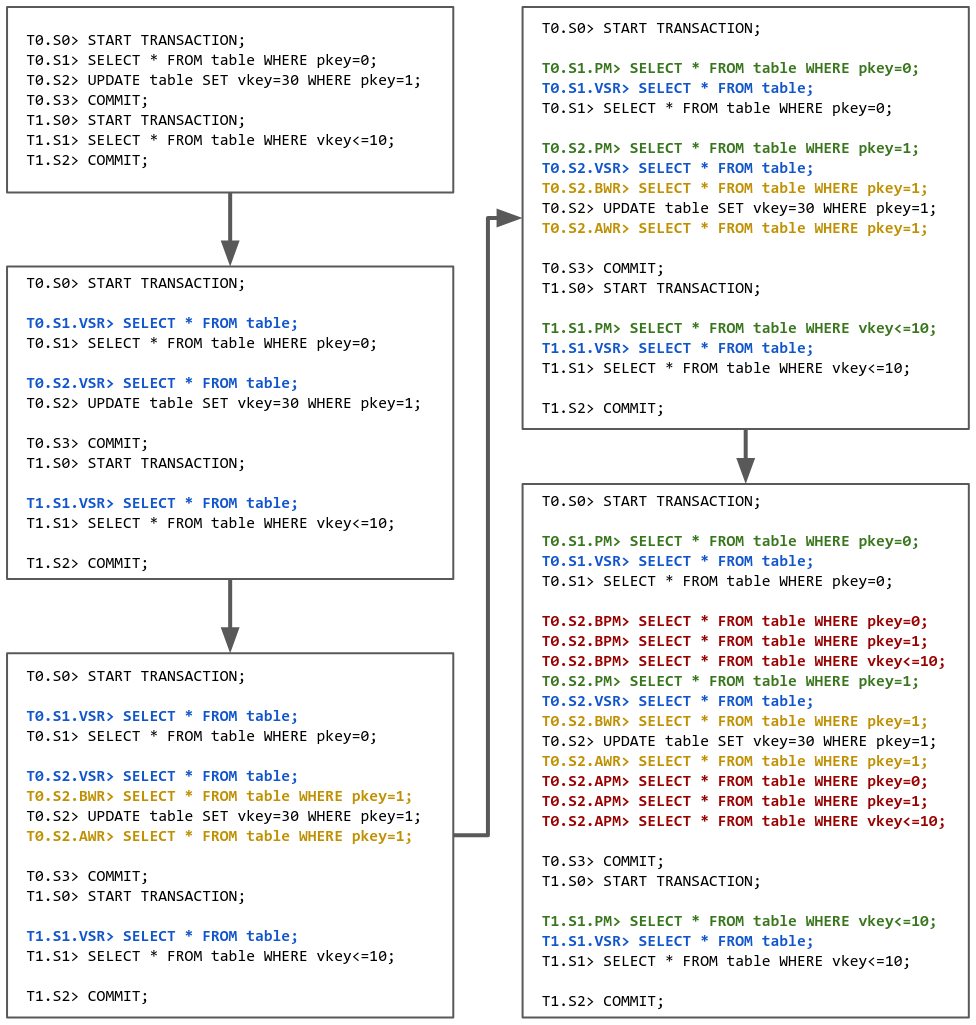
\includegraphics[width=\linewidth]{assets/sql_instrumentation_sample.png}
    \caption{Instrumentation of a (simplified) test case.}
    \label{fig:sql_instrumentation_sample}
\end{figure}



\section{Extracting the DSG with SQL Instrumentation}

\subsection{Methodology}

Our tool is based on \textit{TxCheck} \cite{jiang2023detecting}, which we modify to suit our needs. Our dependency extraction process is thus similar to the one used in \textit{TxCheck}, with slight modification, which are centered around anti-dependencies. As such, we will not go into detail about the direct read dependencies, direct item anti-dependencies, and direct item write dependencies, as they are similar to the ones used by Jiang, Z. \cite{jiang2023detecting}, where a complete and sound technique for extracting them is described, and will focus on the direct predicate anti dependencies and predicate write dependencies.

Given a test case consisting of intertwined transactions, we do the following:

\begin{itemize}
    \item Add instrumentation statements to the SQL queries.
    \item Ensure that the instrumentation code is not interrupted by locking or other operations.
    \item Run the test case, saving the results of the \textit{SELECT} statements.
    \item Extract the DSG edges with the help of the instrumentation results. 
\end{itemize}

The \textit{Predicate Match}, \textit{Before Predicate Match} and \textit{After Predicate Match} statements are used to extract the \textit{Overwrites}, which happen when a transaction overwrites the predicate of another transaction (see definition \ref{def:overwriting}).

\subsection{Extracting Overwrites}

For any two statements $A$ and $B$, where $A$ is a write operation and $B$ contains a predicate, we can check if $A$ \textit{overwrites} $B$ if there exist a primary $pk$ such that:
\begin{itemize}
    \item The \textit{After Write Read} instrumentation of $A$ contains a record with the primary key $pk$ and a version key $v$.
    \item The \textit{Version Set Read} instrumentation of $B$ contains a record with the primary key $pk$ and a version $v'$ such that $v'$ happens before $v$ in the list of versions for the primary key $pk$.
    \item The \textit{Before Predicate Match} instrumentation of $A$ for the predicate of $B$ and the \textit{Predicate Match} instrumentation of $B$ contain $pk$, but the \textit{After Predicate Match} instrumentation of $A$ for the predicate of $B$ does not, or the other way around.
\end{itemize}

Note that if $B$ contains multiple predicates, we need to check for each predicate if $A$ overwrites $B$.

\begin{proof}
We prove that our method for extracting overwrites is both sound and complete.

\textit{Soundness}: If we flag $A$ as \textit{overwriting} $B$, then there exists a primary $pk$ and two versions $v$ and $v'$ such that $v$ is the version of $pk$ installed by $A$, $v'$ is the version of $pk$ present in the version set of $B$, and $v$ happens after $v'$ in the list of versions for $pk$. Furthermore, the \textit{Before Predicate Match} instrumentation of $A$ for the predicate of $B$ contains $pk$, but the \textit{After Predicate Match} instrumentation of $A$ for the predicate of $B$ does not, or the other way around, meaning that $A$ makes $pk$ no longer match the predicate of $B$ or the other way around. This is the definition of an \textit{overwrite}.

\textit{Completeness}: If $A$ overwrites $B$, then there exists a record $x$ for which $A$ installs a version later than the one seen by $B$, and the two versions do not match the predicate of $B$. Let us denote the primary key of $x$ as $pk$, the version installed by $A$ as $v$, and the version seen by $B$ as $v'$. Then, $v$ happens after $v'$ in the list of versions for $pk$, and the \textit{Before Predicate Match} instrumentation of $A$ for the predicate of $B$ contains $pk$. However, the \textit{After Predicate Match} instrumentation of $A$ for the predicate of $B$ does not, or the other way around. This means that our technique correctly identifies $A$ as overwriting $B$.
\end{proof}

\subsection{Extracting Predicate Write Dependencies}

We proved that we are able to check if one statement overwrites another in a sound and complete manner. This allows us to trivially extract \textit{direct predicate anti-dependencies} by checking if a write statement overwrites the predicate of a read statement.

\begin{proof}
    Let $A$ be a write statement and $B$ be a read statement. If $A$ overwrites $B$, then the transaction containing $A$ by definition \textit{directly predicate anti-depends} on the transaction containing $B$.
\end{proof}

\subsection{Extracting Direct Predicate Write Dependencies}

In a similar way, we can extract the \textit{direct predicate write dependencies} by checking that:
\begin{itemize}
    \item The \textit{After Write Read} of a transaction intersects with the \textit{Version Set Read} of a predicated write statement of another transaction, or
    \item One transaction overwrites the predicate of another write transaction.
\end{itemize}

\begin{proof}
    We prove that our method for extracting direct predicate write dependencies is both sound and complete.

    \textit{Soundness}: If we flag $A$ as \textit{directly predicate write-depending} on $B$, then:
    \begin{itemize}
        \item The \textit{After Write Read} of $A$ intersects with the \textit{Version Set Read} of $B$, and $B$ is a predicated write. This means that $A$ installs a version that is read by $B$, so $A$ \textit{directly predicate write-depends} on $B$, or
        \item $A$ overwrites the predicate of $B$, so $A$ \textit{directly predicate write-depends} on $B$.
    \end{itemize}

    \textit{Completeness}: If $A$ \textit{directly predicate write-depends} on $B$, then:
    \begin{itemize}
        \item $A$ installs a version that is read by $B$, which means that the \textit{After Write Read} of $A$ intersects with the \textit{Version Set Read} of $B$, so we flag $A$ as \textit{directly predicate write-depending} on $B$, or
        \item $A$ overwrites the predicate of $B$, so we flag $A$ as \textit{directly predicate write-depending} on $B$.
    \end{itemize}
\end{proof}

\section{Implementation and Results}

We implement our technique on top of \textit{TxCheck}, which we modify to suit our needs. As we are only looking for isolation bugs, we do not need to run the single-transaction \textit{TxCheck} uses as an oracle, so we bypass that part of the code.

The main changes we make to \textit{TxCheck} are:
\begin{itemize}
    \item Update the project to bring it to a working state: \textit{TxCheck} relies on \textit{Docker} images of \textit{Ubuntu 20.04}, on which some dependencies of the project are not available. We fix the broken dependencies, and make the project runnable.
    \item Add the new \textit{Before Predicate Match}, \textit{After Predicate Match} and \textit{Predicate Match} instrumentation types.
    \item Modify the dependency extraction code to create a complete and sound extraction of the DSG dependencies.
    \item Modify the bug minimization code to include support for the new instrumentation types.
    \item Add additional tests based on Adya's theory \cite{adya1999weak} for detecting isolation bugs, which were not previously possible due to the sporadic dependencies created by the original technique.
\end{itemize}

The fuzzing approach of our technique is similar to the one used by \textit{TxCheck}, with the main difference being the ability to extract the DSG dependencies accurately, thus making the \textit{graph de-cycling} phase of \textit{TxCheck}, used to remove circular dependencies assumed to be false positives, unnecessary. This means that, while our approach and \textit{TxCheck} share most of the implementation and work in a similar way, the two are quite different in the way they find bugs:
\begin{itemize}
    \item Our approach relies on properties of the DSG to find isolation bugs.
    \item \textit{TxCheck} checks a few properties of the DSG, but mainly relies on the single-transaction oracle to find bugs, as the DSG extraction used is not sound.
\end{itemize}

\section{Limitations and Future Work}

Our technique is a complete and sound method of extracting of the DSG dependencies, and a step forward in the direction of behavior-based DBMS testing. However, it suffers from similar limitations as the original technique used by \textit{TxCheck}:
\begin{itemize}
    \item The fuzzing is quite slow, with the test case generation and finding a non-blocking schedule being the bottleneck.
    \item While our technique is able to run under any of the isolation levels supported by the DBMS, the lower the isolation level the less checks we can perform, as the DSG has fewer restrictions. In particular, the \textit{Read Uncommitted} isolation level imposes almost no restrictions on the DSG, which makes it hard to find bugs.
    \item Similarly to the original \textit{TxCheck} technique, scheduling for some valid executions might fail due to the additional locking created by the instrumentation.
\end{itemize}

We only implemented support \textit{SELECT}, \textit{UPDATE} and \textit{INSERT} statements. However, support for the \textit{DELETE} statements is also possible. The main caveat is that \textit{DELETE} removes entries from tables, while the Adya model assumes that deleted rows enter an \textit{erased} state, in which they still exist belong in \textit{Version Sets}. This can be solved by:
\begin{itemize}
    \item Having a \textit{deleted} copy of each table, initially empty.
    \item Before a \textit{DELETE} statement, inserting the deleted rows in the \textit{deleted} table.
    \item When performing the \textit{Version Set Read} instrumentation, also reading the entries from the \textit{deleted} table.
\end{itemize}

\section{Conclusion}

In this project, we improve the DSG extraction technique used by \textit{TxCheck}, by adapting the SQL-level instrumentation technique introduced by Jiang, Z. \cite{jiang2023detecting} to obtain a complete and sound list dependency. We implement the changes in the \textit{TxCheck} project, giving \textit{TxCheck} the ability to extract the DSG edges accurately.

While we did not have the time to run a full evaluation of our technique and to let the fuzzing run for a long time, we believe that our technique is a step forward in the direction of behavior-based DBMS testing, and that it has the potential to find more isolation bugs than the original technique used by \textit{TxCheck}.

\input{Conclusions}

\printbibliography

\appendix

% 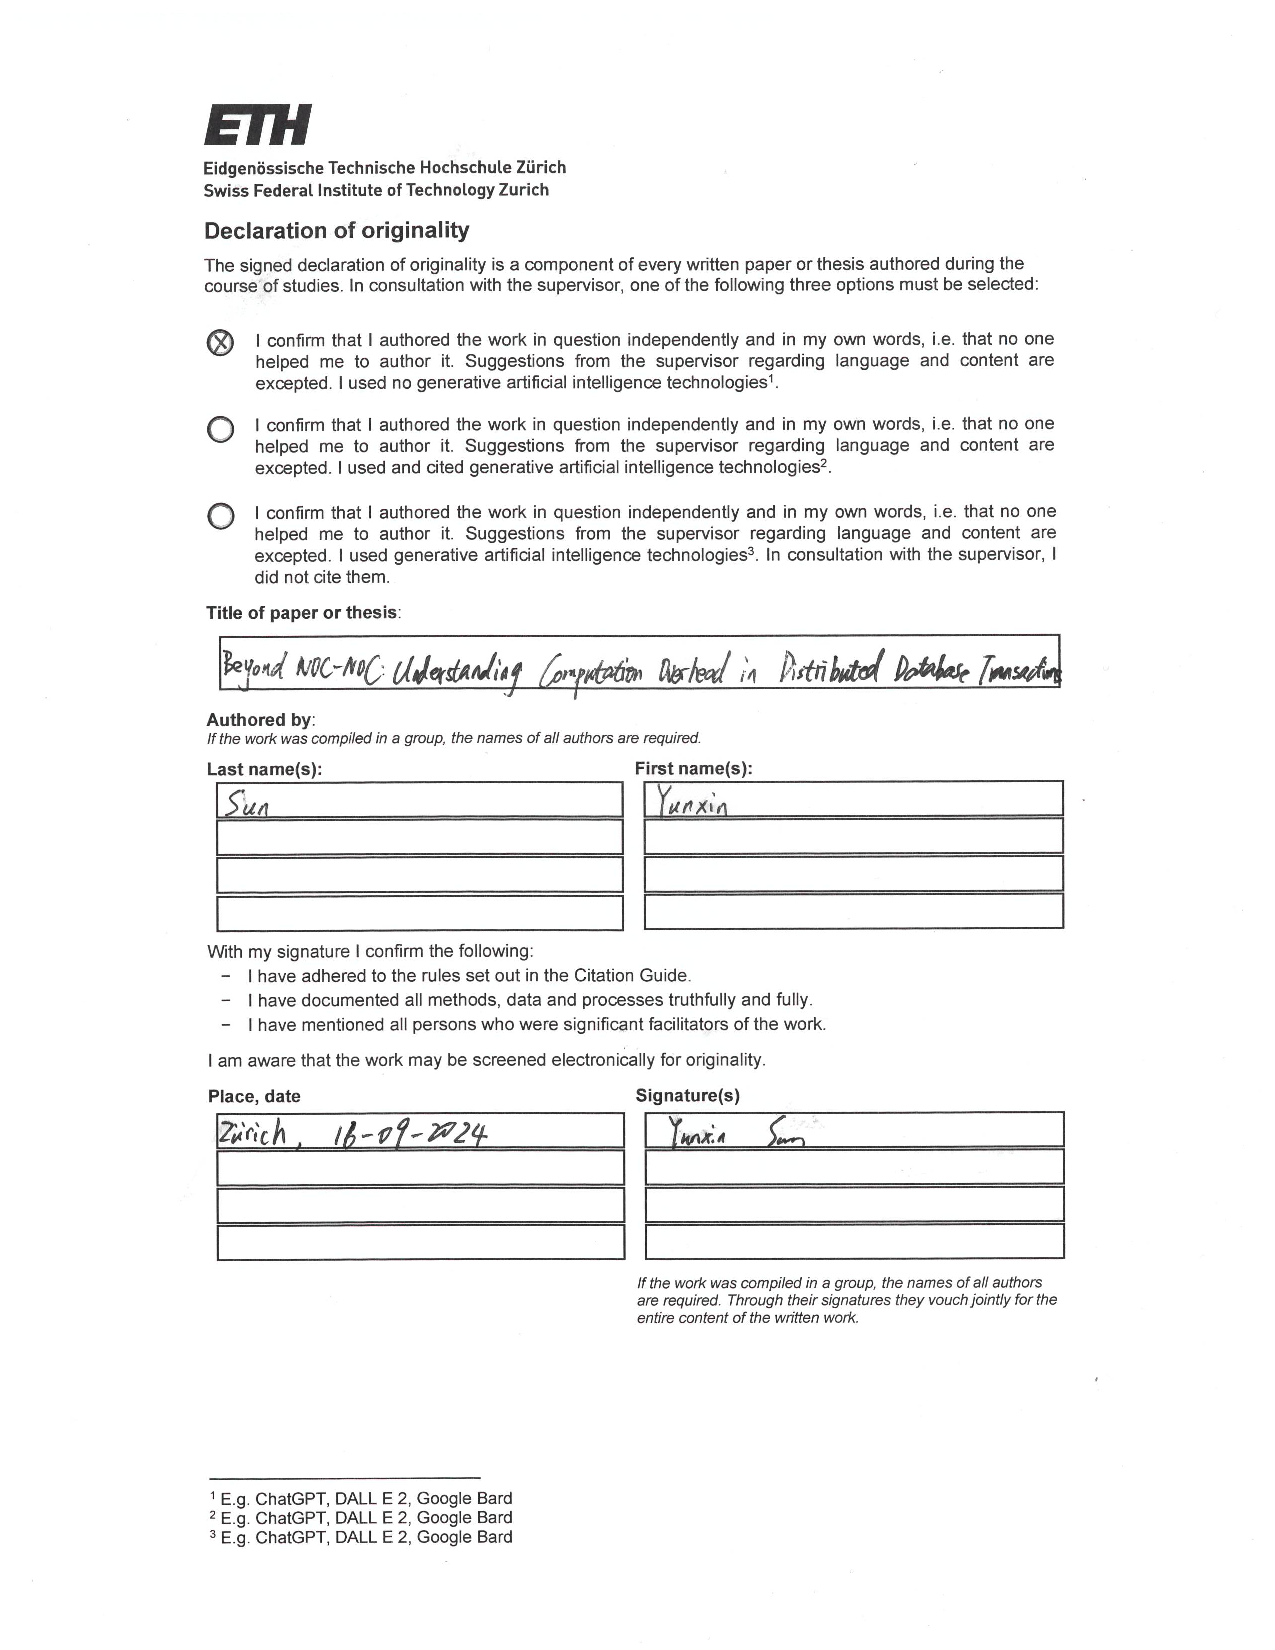
\includepdf[pages={-}]{eth-template/declaration-originality.pdf}

\end{document}
